\documentclass[12pt,a4paper]{article}
\usepackage[a4paper, margin=0.8in, headheight=14pt]{geometry}
\usepackage{fontspec}
\usepackage{unicode-math}
\setmainfont{TeX Gyre Pagella}
\setmonofont[Scale=0.88]{TeX Gyre Cursor}
\setmathfont{Latin Modern Math}
\usepackage{xcolor}
\usepackage{colortbl}
\usepackage{titlesec}
\usepackage{enumitem}
\usepackage{tabularx}
\usepackage{booktabs}
\usepackage{array}
\usepackage{amsmath}
\allowdisplaybreaks
\usepackage{tikz}
\usetikzlibrary{shapes.geometric, arrows.meta, positioning, calc, fit, decorations.pathreplacing, decorations.pathmorphing, patterns, backgrounds}
% circuitikz not required for this subject
\usepackage{tcolorbox}
\tcbuselibrary{skins, breakable}
\usepackage{etoolbox}
\usepackage{hyperref}
\usepackage{fancyhdr}
\usepackage{graphicx}
\usepackage{microtype}
\hyphenpenalty=10000
\exhyphenpenalty=10000
\sloppy
\usepackage{caption}
\usepackage{setspace}
\usepackage{multirow}
\usepackage{tocloft}
\newcommand{\Q}[1]{\textbf{#1}\par\noindent\ignorespaces}
\definecolor{myred}{RGB}{196,30,58}
\definecolor{mydark}{RGB}{30,30,50}
\definecolor{mygreen}{RGB}{14,120,80}
\definecolor{myteal}{RGB}{0,130,140}
\definecolor{myamber}{RGB}{180,100,0}
\definecolor{mypurple}{RGB}{100,30,160}
\definecolor{mygray}{RGB}{246,247,249}
\definecolor{mgframe}{RGB}{180,185,200}
\definecolor{watermark}{RGB}{145,150,170}
\definecolor{hdrred}{RGB}{250,232,235}
\definecolor{hdrgreen}{RGB}{220,244,233}
\definecolor{hdrteal}{RGB}{220,242,244}
\definecolor{hdramber}{RGB}{253,242,215}
\definecolor{hdrpurple}{RGB}{238,228,255}
\definecolor{hdrgray}{RGB}{238,240,245}
\definecolor{rowalt}{RGB}{250,251,253}
\AfterEndEnvironment{tcolorbox}{\color{mydark}}

\titleformat{\section}{\large\bfseries\color{myred}}{\thesection.}{0.5em}{}[\vspace{1pt}{\color{myred}\rule{\linewidth}{0.8pt}}]
\titleformat{\subsection}{\normalsize\bfseries\color{myteal}}{\thesubsection}{0.5em}{}
\titlespacing*{\section}{0pt}{18pt}{7pt}
\titlespacing*{\subsection}{0pt}{11pt}{4pt}
\setlength{\parindent}{0pt}
\setlength{\parskip}{4pt}
\renewcommand{\cfttoctitlefont}{\large\bfseries\color{myred}}
\renewcommand{\cftaftertoctitle}{\par\noindent{\color{myred}\rule{\linewidth}{0.8pt}}}
\setlength{\cftbeforetoctitleskip}{0pt}
\setlength{\cftaftertoctitleskip}{6pt}
\renewcommand{\cftsecfont}{\normalsize\bfseries\color{mydark}}
\renewcommand{\cftsecpagefont}{\normalsize\bfseries\color{mydark}}
\renewcommand{\cftsecleader}{\cftdotfill{\cftdotsep}}
\setlength{\cftbeforesecskip}{7pt}
\renewcommand{\cftsubsecfont}{\small\color{mydark}}
\renewcommand{\cftsubsecpagefont}{\small\color{mydark}}
\setlength{\cftbeforesubsecskip}{3pt}
\setlength{\cftsubsecindent}{1.4em}
\renewcommand{\cftpartfont}{\normalsize\bfseries\color{myteal}}
\renewcommand{\cftpartpagefont}{\normalsize\bfseries\color{myteal}}
\setlength{\cftbeforepartskip}{14pt}
\renewcommand{\arraystretch}{1.45}
\setlength{\tabcolsep}{6pt}
\arrayrulecolor{mydark}
\newcolumntype{B}[1]{>{\small\bfseries\raggedright\arraybackslash}m{#1}}
\newcolumntype{C}[1]{>{\centering\arraybackslash}m{#1}}
\newcolumntype{Y}{>{\small\raggedright\arraybackslash}X}
\renewcommand{\tabularxcolumn}[1]{m{#1}}
\newcommand{\currmodule}{Module 1}
\pagestyle{fancy}
\fancyhf{}
\fancyhead[L]{\small\color{myred}\textbf{EC402}\;\color{mydark}--- Analog Circuits}
\fancyhead[R]{\small\color{myteal}\textbf{\currmodule\ Notes}}
\fancyfoot[C]{\small\color{mydark}\thepage}
\fancyfoot[R]{\small\color{watermark}\textit{\copyright\ Biraj}}
\renewcommand{\headrulewidth}{0.5pt}
\renewcommand{\footrulewidth}{0.3pt}

\hypersetup{colorlinks=true, linkcolor=myteal, urlcolor=myteal,
  pdfauthor={Biraj Sarkar},
  pdftitle={EC402 --- Combined Notes}}

\tcbset{
  tikzbox/.style={
    colback=mygray, colframe=mgframe, boxrule=0.6pt, arc=4pt,
    left=8pt, right=8pt, top=6pt, bottom=6pt,
    colbacktitle=mgframe, coltitle=mydark, fonttitle=\small\bfseries
  },
  defbox/.style={
    colback=hdrgreen, colframe=mygreen, boxrule=0.8pt, arc=4pt,
    left=9pt, right=9pt, top=6pt, bottom=6pt,
    colbacktitle=mygreen, coltitle=white, fonttitle=\small\bfseries
  },
  formulabox/.style={
    colback=hdrteal, colframe=myteal, boxrule=0.8pt, arc=4pt,
    left=9pt, right=9pt, top=7pt, bottom=7pt,
    colbacktitle=myteal, coltitle=white, fonttitle=\small\bfseries
  },
  examplebox/.style={
    colback=hdramber, colframe=myamber, boxrule=0.8pt, arc=4pt,
    left=9pt, right=9pt, top=6pt, bottom=6pt,
    colbacktitle=myamber, coltitle=white, fonttitle=\small\bfseries
  },
  masonbox/.style={
    colback=hdrpurple, colframe=mypurple, boxrule=0.8pt, arc=4pt,
    left=9pt, right=9pt, top=6pt, bottom=6pt,
    colbacktitle=mypurple, coltitle=white, fonttitle=\small\bfseries
  },
  exambox/.style={
    colback=hdrpurple, colframe=mypurple, boxrule=1pt, arc=5pt,
    left=10pt, right=10pt, top=8pt, bottom=8pt,
    colbacktitle=mypurple, coltitle=white, fonttitle=\bfseries,
    breakable, title after break={\textbf{Frequently Asked / Viva Questions (contd.)}}
  }
}
\tcbset{breakable}
\tcbset{coltext=mydark}
\tcbset{after={\color{mydark}}}

\tikzset{
  block/.style={rectangle, draw=myteal, fill=hdrteal,
    text width=2.4cm, align=center, minimum height=0.95cm,
    font=\small, rounded corners=3pt, line width=0.7pt},
  redblock/.style={rectangle, draw=myred, fill=hdrred,
    text width=2.4cm, align=center, minimum height=0.95cm,
    font=\small, rounded corners=3pt, line width=0.7pt},
  sumjunc/.style={circle, draw=myamber, fill=hdramber,
    minimum size=0.62cm, font=\small, line width=0.8pt},
  arrow/.style={-Stealth, thick, color=mydark},
  redarrow/.style={-Stealth, thick, color=myred},
  line/.style={thick, color=mydark}
}

\newcommand{\modulestart}[2]{%
  \clearpage
  \renewcommand{\currmodule}{Module #1}%
  \renewcommand{\theHsection}{mod#1.\arabic{section}}%
  \renewcommand{\theHsubsection}{\theHsection.\arabic{subsection}}%
  \renewcommand{\theHsubsubsection}{\theHsubsection.\arabic{subsubsection}}%
  \phantomsection
  \addcontentsline{toc}{part}{Module #1: #2}%
  \setcounter{section}{0}%
  \begin{center}
    \vspace*{1.0cm}
    {\Huge\bfseries\color{myred} Module #1}\\[10pt]
    {\Large\bfseries\color{mydark} #2}\\[10pt]
    {\color{myred}\rule{0.55\linewidth}{1.2pt}}
  \end{center}
  \vspace{14pt}
}
\begin{document}

\thispagestyle{empty}

% ─── Page Border (TikZ Overlay) ────────────────────────────────────────────────
\begin{tikzpicture}[remember picture, overlay]
  % Outer border (fine line in mgframe)
  \draw[color=mgframe, line width=1.5pt] 
    ($(current page.north west) + (0.6in, -0.6in)$) rectangle 
    ($(current page.south east) + (-0.6in, 0.6in)$);
  % Inner border (finer accent line in myred)
  \draw[color=myred, line width=0.8pt] 
    ($(current page.north west) + (0.65in, -0.65in)$) rectangle 
    ($(current page.south east) + (-0.65in, 0.65in)$);
\end{tikzpicture}

\vspace*{1.0cm}
\begin{center}
  {\Huge\bfseries\color{myred} EC402}\\[10pt]
  {\LARGE\bfseries\color{mydark} Analog Circuits}\\[20pt]
  {\color{myred}\rule{0.7\linewidth}{1.5pt}}\\[18pt]
  {\Large\color{myteal}\textbf{Combined Module Notes}}\\[8pt]
  {\large\color{mydark} Modules 1 -- 4}\\[40pt]
  {\normalsize\color{mydark} Semester IV \quad$\bullet$\quad ECE \quad$\bullet$\quad 3 Credits}\\[12pt]
  {\normalsize\color{mydark} CGEC \;$|$\; B.Tech ECE (2023--27)}
\end{center}
\vspace{1.0cm}
\begin{center}
  \begin{tcolorbox}[colback=mygray, colframe=mgframe, boxrule=0.5pt, arc=3pt, width=0.85\linewidth]
    \centering\small\color{mydark}
    \textbf{Disclaimer / Study Guide Notice:}\\
    These are condensed \textbf{Short Notes} focusing on core theory, key formulas, block/circuit diagrams, and standard viva Q\&As for university exam revision. Exhaustive numerical practice problems and derivation edge cases are not covered. This serves as a quick-revision reference guide for students.
  \end{tcolorbox}
\end{center}
\vfill
\vspace{0.6cm}
\begin{center}
  {\large\bfseries\color{mypurple} Biraj Sarkar}\\[16pt]
  {\footnotesize\color{watermark}\textbf{IN ASSOCIATION WITH}}\\[8pt]
  {\small\bfseries\color{mydark} MAKAUT Wingman \quad$\bullet$\quad MAKAUT Future Minds}\\[12pt]
  {\large\bfseries\color{myteal} Cooch Behar Government Engineering College}
\end{center}
\vfill
\begin{center}{\small\color{watermark}\textit{Exam-Ready Notes}}\end{center}
\clearpage

\hypersetup{linkcolor=mydark}
\tableofcontents
\hypersetup{linkcolor=myteal}
\clearpage

% -- Module 1 -----------------------------------------------------------------
\modulestart{1}{Diode Circuits: Rectifiers, Filters, Clippers and Clampers}

\section{Diode Circuits: Rectifiers, Filters, Clippers and Clampers}

\begin{tcolorbox}[defbox, title={Rectifier Fundamentals}]
A \textbf{rectifier} is a non-linear circuit converting alternating voltage ($ac$) to unidirectional pulsating direct voltage ($dc$) utilizing the unilateral conduction of $p$-$n$ junction diodes. The performance of rectifiers is governed by rectification efficiency $\eta$, ripple factor $\gamma$, Transformer Utilization Factor ($\mathrm{TUF}$), and Peak Inverse Voltage ($\mathrm{PIV}$).
\end{tcolorbox}

\subsection{Half-Wave and Full-Wave Rectifiers}
Consider an input $v_i(t) = V_m\sin(\omega t)$ applied across a load resistance $R_L$ with diode forward resistance $r_f$.

\begin{enumerate}[leftmargin=1.5em, itemsep=3pt]
  \item \textbf{Half-Wave Rectifier (HWR)}: Conducts only during positive half cycles ($0 \le \omega t \le \pi$):
  \[
  \begin{aligned}
  I_{dc} &= \frac{1}{2\pi}\int_0^\pi I_m\sin\theta\,d\theta = \frac{I_m}{\pi},\qquad V_{dc} = I_{dc}R_L = \frac{V_m}{\pi},\\
  I_{rms} &= \sqrt{\frac{1}{2\pi}\int_0^\pi I_m^2\sin^2\theta\,d\theta} = \frac{I_m}{2},\qquad V_{rms} = \frac{V_m}{2}.
  \end{aligned}
  \]
  \item \textbf{Full-Wave Rectifier (Center-Tapped and Bridge)}: Conducts during both half cycles:
  \[
  \begin{aligned}
  I_{dc} &= \frac{1}{\pi}\int_0^\pi I_m\sin\theta\,d\theta = \frac{2I_m}{\pi},\qquad V_{dc} = \frac{2V_m}{\pi},\\
  I_{rms} &= \sqrt{\frac{1}{\pi}\int_0^\pi I_m^2\sin^2\theta\,d\theta} = \frac{I_m}{\sqrt{2}},\qquad V_{rms} = \frac{V_m}{\sqrt{2}}.
  \end{aligned}
  \]
\end{enumerate}

\begin{tcolorbox}[formulabox, title={Performance Metrics of Rectifiers}]
\begin{enumerate}[leftmargin=1.5em, itemsep=2pt]
  \item \textbf{Ripple Factor ($\gamma$)}: Ratio of effective $ac$ component to the average $dc$ level:
  \[
  \gamma = \frac{V_{ac,rms}}{V_{dc}} = \sqrt{\left(\frac{I_{rms}}{I_{dc}}\right)^2 - 1}.
  \]
  For HWR: $\gamma = \sqrt{(\pi/2)^2 - 1} \approx 1.21$. For FWR: $\gamma = \sqrt{(\pi/(2\sqrt{2}))^2 - 1} \approx 0.482$.
  \item \textbf{Rectification Efficiency ($\eta$)}: Ratio of $dc$ output power to total $ac$ input power:
  \[
  \eta = \frac{P_{dc}}{P_{ac}} = \frac{I_{dc}^2 R_L}{I_{rms}^2 (R_L + r_f)}.
  \]
  For HWR: $\eta_{\max} = \frac{4}{\pi^2} \approx 40.6\%$. For FWR: $\eta_{\max} = \frac{8}{\pi^2} \approx 81.2\%$.
  \item \textbf{Transformer Utilization Factor ($\mathrm{TUF}$)}: $\mathrm{TUF} = P_{dc} / V_{\text{rated}}I_{\text{rated}}$.
  $\mathrm{TUF}_{\mathrm{HWR}} = 0.287$, $\mathrm{TUF}_{\mathrm{FWR,Center}} = 0.693$, $\mathrm{TUF}_{\mathrm{Bridge}} = 0.812$.
  \item \textbf{Peak Inverse Voltage ($\mathrm{PIV}$)}: Maximum reverse bias voltage appearing across a non-conducting diode:
  $\mathrm{PIV}_{\mathrm{HWR}} = V_m$, $\mathrm{PIV}_{\mathrm{Center-Tapped}} = 2V_m$, $\mathrm{PIV}_{\mathrm{Bridge}} = V_m$.
\end{enumerate}
\end{tcolorbox}

\par\vspace{6pt}\noindent
\begin{tabularx}{\linewidth}{|B{3.4cm}|Y|Y|Y|}
\hline
\textbf{Parameter} & \textbf{Half-Wave Rectifier} & \textbf{Center-Tapped FWR} & \textbf{Bridge Rectifier} \\
\hline
\textbf{Number of Diodes} & 1 & 2 & 4 \\
\hline
\textbf{$dc$ Voltage ($V_{dc}$)} & $V_m/\pi \approx 0.318 V_m$ & $2V_m/\pi \approx 0.636 V_m$ & $2V_m/\pi \approx 0.636 V_m$ \\
\hline
\textbf{Ripple Factor ($\gamma$)} & $1.21$ ($121\%$ ripple) & $0.482$ ($48.2\%$ ripple) & $0.482$ ($48.2\%$ ripple) \\
\hline
\textbf{Efficiency ($\eta_{\max}$)}& $40.6\%$ & $81.2\%$ & $81.2\%$ \\
\hline
\textbf{Ripple Frequency} & $f_{in}$ ($50\,\mathrm{Hz}$) & $2f_{in}$ ($100\,\mathrm{Hz}$) & $2f_{in}$ ($100\,\mathrm{Hz}$) \\
\hline
\textbf{Peak Inverse Voltage} & $V_m$ & $2V_m$ & $V_m$ \\
\hline
\textbf{Center-Tap Required}& No & Yes (bulky transformer) & No \\
\hline
\end{tabularx}
\par\vspace{12pt}

\subsection{Power Supply Smoothing Filters}
Smoothing filters suppress $ac$ ripple harmonics leaving pure $dc$:
\begin{enumerate}[leftmargin=1.5em, itemsep=2pt]
  \item \textbf{Shunt Capacitor Filter ($C$-Filter)}: Capacitor charges to $V_m$ on peaks and discharges slowly into $R_L$ with time constant $R_L C \gg T/2$. Ripple factor for FWR: $\gamma \approx \frac{1}{4\sqrt{3} f R_L C}$.
  \item \textbf{Series Inductor Filter ($L$-Filter)}: Opposes sudden current changes: $\gamma \approx \frac{R_L}{3\sqrt{2}\omega L}$. Suitable for heavy loads (small $R_L$).
  \item \textbf{Choke-Input ($LC$) Filter}: Combines series $L$ and shunt $C$: $\gamma \approx \frac{\sqrt{2}}{3}\frac{X_C}{X_L} = \frac{1}{6\sqrt{2}\omega^2 L C}$, independent of load resistance $R_L$. Critical inductance: $L_c \ge R_L / (3\omega)$.
  \item \textbf{$\pi$-Filter ($CLC$-Filter)}: Yields lowest ripple: $\gamma \approx \frac{\sqrt{2}}{8\omega^3 C_1 C_2 L R_L}$, but high diode surge current.
\end{enumerate}

\subsection{Clippers (Limiters) and Clampers (DC Restorers)}
\begin{itemize}[leftmargin=1.5em, itemsep=3pt]
  \item \textbf{Clippers}: Waveform-shaping circuits that remove portions of an applied signal above or below preset reference levels without distorting the remaining part. Implemented as series clippers (diode in series with signal path) or shunt clippers (diode in parallel across load).
  \item \textbf{Two-Level (Slicer) Clipper}: Two diodes biased with opposite reference voltages ($V_{R1}, V_{R2}$) clip both positive and negative peaks, generating trapezoidal or square waves from a sine wave.
  \item \textbf{Clampers}: Circuits that shift the entire waveform up or down to a different $dc$ level without altering the peak-to-peak amplitude. Requires a diode, capacitor, and resistor satisfying $R_L C \ge 10T$.
  \item \textbf{Clamping Theorem}: At steady state, ratio of area under positive curve ($A_+$) to negative curve ($A_-$) equals ratio of forward resistance to load resistance: $A_+ / A_- = r_f / R_L$.
\end{itemize}

\begin{tcolorbox}[tikzbox, unbreakable, title={Diode Clipper and Clamper Topologies}]
\centering
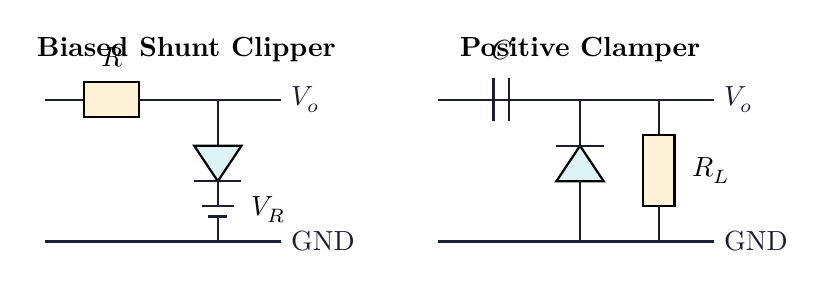
\begin{tikzpicture}[x=1cm,y=0.9cm]
  % Shunt Clipper
  \node[above] at (1.8,2.4) {\bfseries Biased Shunt Clipper};
  \draw[line] (0,2)--(1.5,2);
  \draw[thick,fill=hdramber] (0.5,1.75) rectangle (1.2,2.25);
  \node[above=2pt] at (0.85,2.25) {$R$};
  \draw[line] (1.2,2)--(3,2) node[right] {$V_o$};
  \draw[line] (0,0)--(3,0) node[right] {GND};
  \draw[line] (2.2,2)--(2.2,1.35);
  \draw[thick,fill=hdrteal] (1.9,1.35)--(2.5,1.35)--(2.2,0.85)--cycle;
  \draw[line] (1.9,0.85)--(2.5,0.85);
  \draw[line] (2.2,0.85)--(2.2,0.5);
  \draw[line] (2.0,0.5)--(2.4,0.5);
  \draw[line] (2.08,0.35)--(2.32,0.35);
  \draw[line] (2.2,0.35)--(2.2,0);
  \node[right=3pt] at (2.4,0.45) {$V_R$};

  % Positive Clamper
  \node[above] at (6.8,2.4) {\bfseries Positive Clamper};
  \draw[line] (5,2)--(6,2);
  \draw[line] (5.7,2.3)--(5.7,1.7);
  \draw[line] (5.9,2.3)--(5.9,1.7);
  \node[above=3pt] at (5.8,2.3) {$C$};
  \draw[line] (5.9,2)--(8.5,2) node[right] {$V_o$};
  \draw[line] (5,0)--(8.5,0) node[right] {GND};
  \draw[line] (6.8,2)--(6.8,1.35);
  \draw[thick,fill=hdrteal] (6.5,0.85)--(7.1,0.85)--(6.8,1.35)--cycle;
  \draw[line] (6.5,1.35)--(7.1,1.35);
  \draw[line] (6.8,0.85)--(6.8,0);
  \draw[line] (7.8,2)--(7.8,1.5);
  \draw[thick,fill=hdramber] (7.6,0.5) rectangle (8.0,1.5);
  \node[right=3pt] at (8.0,1.0) {$R_L$};
  \draw[line] (7.8,0.5)--(7.8,0);
\end{tikzpicture}\par
\small Shunt clipper limits peaks above $V_R + V_D$. The positive clamper shifts the signal upwards so that its negative peaks rest at $0\,\mathrm{V}$.
\end{tcolorbox}

\section{Two-Port Amplifier Models and Loading Effects}

\begin{tcolorbox}[defbox, title={The Four Fundamental Amplifier Models}]
Amplifiers are linear two-port networks characterized by input resistance $R_i$, open-circuit or short-circuit gain parameter, and output resistance $R_o$:
\begin{enumerate}[leftmargin=1.5em, itemsep=2pt]
  \item \textbf{Voltage Amplifier}: $V_o = A_{vo} V_i$. Ideal: $R_i \to \infty$, $R_o = 0$.
  \item \textbf{Current Amplifier}: $I_o = A_{is} I_i$. Ideal: $R_i = 0$, $R_o \to \infty$.
  \item \textbf{Transconductance Amplifier}: $I_o = G_m V_i$. Ideal: $R_i \to \infty$, $R_o \to \infty$.
  \item \textbf{Transresistance Amplifier}: $V_o = R_m I_i$. Ideal: $R_i = 0$, $R_o = 0$.
\end{enumerate}
\end{tcolorbox}

\subsection{Source and Load Resistance Loading Effects}
When connected between an actual source ($V_s, R_s$) and a real load $R_L$:
\[
V_i = V_s \left(\frac{R_i}{R_s + R_i}\right),\qquad
V_o = A_{vo} V_i \left(\frac{R_L}{R_o + R_L}\right) = A_{vo} V_s \left(\frac{R_i}{R_s + R_i}\right)\left(\frac{R_L}{R_o + R_L}\right).
\]
Effective voltage gain $A_v = V_o/V_s$ drops below intrinsic gain $A_{vo}$ due to input voltage division (when $R_s \not\ll R_i$) and output loading (when $R_L \not\gg R_o$).

\begin{tcolorbox}[examplebox, title={Amplifier Loading Effect Calculation}]
A voltage amplifier has $R_i = 100\,\mathrm{k}\Omega$, $R_o = 50\,\Omega$, and $A_{vo} = 200$. It is driven by a source with $R_s = 25\,\mathrm{k}\Omega$ and drives a load $R_L = 100\,\Omega$.
\[
\begin{aligned}
\text{Input attenuation factor:}\quad \alpha_i &= \frac{R_i}{R_s + R_i} = \frac{100}{25 + 100} = 0.8,\\
\text{Output loading factor:}\quad \alpha_o &= \frac{R_L}{R_o + R_L} = \frac{100}{50 + 100} = 0.667,\\
\text{Overall voltage gain:}\quad A_v &= \frac{V_o}{V_s} = A_{vo}\cdot\alpha_i\cdot\alpha_o = 200(0.8)(0.667) \approx 106.7.
\end{aligned}
\]
Loading degrades the effective amplification from $200$ to $106.7$ ($46.6\%$ loss).
\end{tcolorbox}

\section{Biasing Schemes and Stability Analysis for BJT and FET}

\begin{tcolorbox}[defbox, title={Operating Point ($Q$-Point) and Stability}]
To amplify linear $ac$ signals without clipping, transistors must be biased in the \textbf{Active Region} (BJT: forward-biased emitter junction, reverse-biased collector junction; FET: pinched-off saturation region). The operating point $Q(V_{CEQ}, I_{CQ})$ represents the steady-state $dc$ voltages and currents.
\end{tcolorbox}

\subsection{BJT Biasing Configurations and Stability Factors}
Variations in temperature $T$ cause drift in reverse saturation current $I_{CO}$ (doubles every $10^\circ\mathrm{C}$ rise), base-emitter voltage $V_{BE}$ (decreases by $2.5\,\mathrm{mV/^\circ C}$), and current gain $\beta$. Stability factors define the sensitivity:
\[
S = \frac{\partial I_C}{\partial I_{CO}},\qquad
S' = \frac{\partial I_C}{\partial V_{BE}},\qquad
S'' = \frac{\partial I_C}{\partial \beta}.
\]
General relation: $I_C = \beta I_B + (1+\beta)I_{CO}$. Differentiating with respect to $I_C$:
\[
S = \frac{1 + \beta}{1 - \beta \left(\dfrac{\partial I_B}{\partial I_C}\right)}.
\]

\begin{enumerate}[leftmargin=1.5em, itemsep=3pt]
  \item \textbf{Fixed Bias}: $I_B = (V_{CC} - V_{BE})/R_B$. Since $\partial I_B/\partial I_C = 0$, $S = 1+\beta$. Highly unstable ($S \approx 100$--$300$); thermal runaway occurs readily.
  \item \textbf{Collector-to-Base Feedback Bias}: $I_B = (V_{CC} - V_{BE} - I_C R_C)/(R_B + R_C)$. Provides negative feedback: $\partial I_B/\partial I_C = -R_C/(R_B+R_C) < 0$, giving $S = \frac{1+\beta}{1 + \beta R_C/(R_B+R_C)} < 1+\beta$.
  \item \textbf{Voltage Divider Bias (Self-Bias / Emitter Bias)}: Most robust topology. Applying Thevenin's theorem at the base:
  \[
  V_{th} = V_{CC}\left(\frac{R_2}{R_1+R_2}\right),\qquad R_{th} = R_1 \parallel R_2.
  \]
  Loop equation: $V_{th} = I_B R_{th} + V_{BE} + I_E R_E \approx I_B R_{th} + V_{BE} + (I_B + I_C)R_E$.
  \[
  I_B = \frac{V_{th} - V_{BE} - I_C R_E}{R_{th} + R_E} \implies \frac{\partial I_B}{\partial I_C} = -\frac{R_E}{R_{th} + R_E}.
  \]
  Substituting into the stability factor formula:
  \[
  S = (1+\beta)\frac{1 + R_{th}/R_E}{1+\beta + R_{th}/R_E}.
  \]
  \textit{Condition for Excellent Stability}: If $R_{th}/R_E \ll 1$, then $S \to 1$ (perfect stability independent of $\beta$). Practical rule: $R_{th} \le 0.1(1+\beta)R_E$ and $I_{\mathrm{divider}} \ge 10 I_B$.
\end{enumerate}

\subsection{Thermal Runaway Avoidance}
Collector power dissipation is $P_C \approx V_{CE} I_C$. Temperature rise $\Delta T = \theta P_C$ (where $\theta$ is thermal resistance in $^\circ\mathrm{C/W}$). A cumulative cycle occurs: $T \uparrow \implies I_{CO} \uparrow \implies I_C \uparrow \implies P_C \uparrow \implies T \uparrow$ until destructive breakdown occurs.
\begin{tcolorbox}[formulabox, title={Condition to Prevent Thermal Runaway}]
Thermal runaway is completely prevented if the rate of heat dissipation exceeds the rate of heat generation:
\[
\frac{\partial P_C}{\partial T_j} < \frac{1}{\theta} \iff V_{CE} < \frac{V_{CC}}{2}.
\]
In practice, designing $V_{CEQ} \le V_{CC}/2$ ensures inherent unconditional thermal stability.
\end{tcolorbox}

\subsection{FET Biasing Schemes (JFET and MOSFET)}
For JFETs and depletion MOSFETs, drain current follows Shockley's equation: $I_D = I_{DSS}(1 - V_{GS}/V_P)^2$.
\begin{itemize}[leftmargin=1.5em, itemsep=2pt]
  \item \textbf{Self-Bias}: Gate grounded ($V_G = 0$) via high resistor $R_G$ ($1\,\mathrm{M}\Omega$). Source resistor $R_S$ develops $V_S = I_D R_S$, producing $V_{GS} = -I_D R_S$. The operating point is the intersection of the transfer curve with the $dc$ bias line $I_D = -V_{GS}/R_S$.
  \item \textbf{Voltage Divider Bias}: $V_G = V_{DD}[R_2/(R_1+R_2)]$. Then $V_{GS} = V_G - I_D R_S$, stabilizing $I_{DQ}$ against device parameter variations ($I_{DSS}$ and $V_P$ spreads).
\end{itemize}

\section{Small-Signal Analysis and Low-Frequency Transistor Models}

\subsection{Low-Frequency BJT Models \texorpdfstring{($h$-Parameter and Hybrid-$\pi$)}{(h-Parameter and Hybrid-pi)}}
For small $ac$ excursions around the $Q$-point:
\begin{itemize}[leftmargin=1.5em, itemsep=2pt]
  \item \textbf{$h$-Parameter Model}: $v_1 = h_i i_1 + h_r v_2$, $i_2 = h_f i_1 + h_o v_2$. For CE: $h_{ie}$ (input resistance), $h_{re}$ (reverse voltage feedback), $h_{fe} = \beta$ (forward current gain), $h_{oe}$ (output conductance).
  \item \textbf{Hybrid-$\pi$ Model}: Transconductance $g_m = I_C/V_T$ (where $V_T = k T/q \approx 26\,\mathrm{mV}$ at room temp), base resistance $r_\pi = \beta/g_m = \beta V_T/I_C$, output resistance $r_o = V_A/I_C$ (where $V_A$ is the Early voltage), and emitter intrinsic resistance $r_e = \alpha/g_m \approx V_T/I_E$.
\end{itemize}

\subsection{BJT Amplifier Configurations (CE, CB, CC)}
\begin{tcolorbox}[defbox, title={Common-Terminal BJT Configurations}]
An amplifier configuration is named for the transistor terminal shared by the input and output signal paths. In \textbf{common emitter (CE)}, the input is at the base and the output at the collector. In \textbf{common base (CB)}, the input is at the emitter and the output at the collector. In \textbf{common collector (CC)}, the input is at the base and the output at the emitter.
\end{tcolorbox}

\begin{tcolorbox}[formulabox, title={Analytical Small-Signal Expressions for BJT Amplifiers}, title after break={BJT Amplifier Expressions (contd.)}]
\begin{enumerate}[leftmargin=1.8em, itemsep=8pt]
  \item \textbf{Common Emitter (CE) with Bypass $C_E$}:
  \[
  \begin{aligned}
  A_v &= -g_m (R_C \parallel R_L)
       = -\frac{\beta (R_C \parallel R_L)}{r_\pi}
       \approx -\frac{R_C \parallel R_L}{r_e}, \\[3pt]
  R_i &= R_B \parallel r_\pi, \\[3pt]
  R_o &= R_C \parallel r_o.
  \end{aligned}
  \]
  Provides high inverting voltage gain ($180^\circ$ phase inversion) and high current gain.
  \item \textbf{Common Emitter with Unbypassed Emitter Resistor $R_E$}:
  \[
  \begin{aligned}
  A_v &\approx -\frac{R_C \parallel R_L}{r_e + R_E}, \\[3pt]
      &\approx -\frac{R_C \parallel R_L}{R_E}
        \quad \text{when } R_E \gg r_e, \\[3pt]
  R_i &= R_B \parallel \left[r_\pi + (1+\beta)R_E\right].
  \end{aligned}
  \]
  Degeneration stabilizes voltage gain against temperature and parameter drift at the cost of reduced gain.
  \item \textbf{Common Collector (CC / Emitter Follower)}:
  Let $R_E' = R_E \parallel R_L$ be the loaded emitter resistance and
  $R_s' = R_s \parallel R_B$ be the resistance seen from the base with
  the input source set to zero.
  \[
  \begin{aligned}
  A_v &= \frac{(1+\beta)R_E'}{r_\pi + (1+\beta)R_E'} \approx 1, \\[3pt]
  R_i &= R_B \parallel \left[r_\pi + (1+\beta)R_E'\right], \\[3pt]
  R_o &= R_E \parallel \left(\frac{r_\pi + R_s'}{1+\beta}\right).
  \end{aligned}
  \]
  The near-unity gain, high input resistance and low output resistance
  make this stage useful as a non-inverting buffer.
  \item \textbf{Common Base (CB)}:
  \[
  \begin{aligned}
  A_v &= +g_m (R_C \parallel R_L), & A_i &\approx \alpha \approx 1, \\[3pt]
  R_i &\approx r_e \parallel R_E, & R_o &\approx R_C.
  \end{aligned}
  \]
  For $R_E \gg r_e$, the input resistance is close to $r_e$.
  The stage is non-inverting and is used in high-frequency RF amplifiers.
\end{enumerate}
\end{tcolorbox}

\par\vspace{6pt}\noindent
\begin{tabularx}{\linewidth}{|B{3.2cm}|Y|Y|Y|}
\hline
\textbf{Parameter} & \textbf{Common Emitter (CE)} & \textbf{Common Collector (CC)} & \textbf{Common Base (CB)} \\
\hline
\textbf{Voltage Gain ($A_v$)} & High ($\sim -100$ to $-500$) & Low ($\approx 1$, non-inverting) & High ($\sim +100$ to $+500$) \\
\hline
\textbf{Current Gain ($A_i$)} & High ($\sim \beta \approx 100$) & Highest ($\sim 1+\beta \approx 101$)& Low ($\sim \alpha \approx 0.99$) \\
\hline
\textbf{Input Resistance ($R_i$)}& Moderate ($\sim 1\,\mathrm{k}\Omega$--$5\,\mathrm{k}\Omega$) & Very High ($\sim 100\,\mathrm{k}\Omega$--$500\,\mathrm{k}\Omega$) & Very Low ($\sim 20\,\Omega$--$50\,\Omega$) \\
\hline
\textbf{Output Resistance ($R_o$)}& Moderate ($\sim 10\,\mathrm{k}\Omega$--$50\,\mathrm{k}\Omega$)& Very Low ($\sim 10\,\Omega$--$50\,\Omega$) & High ($\sim 100\,\mathrm{k}\Omega$--$1\,\mathrm{M}\Omega$) \\
\hline
\textbf{Phase Shift} & $180^\circ$ (inverting) & $0^\circ$ (in-phase) & $0^\circ$ (in-phase) \\
\hline
\textbf{Primary Application}& Voltage \& Power Amplification & Impedance Matching / Buffer & High-Frequency RF Amplifier \\
\hline
\end{tabularx}
\par\vspace{12pt}

\subsection{Multistage Amplifiers (Low Frequency)}
When multiple amplifier stages are cascaded ($n$ stages):
\[
A_v = A_{v1} \cdot A_{v2} \cdots A_{vn},\qquad
R_{in} = R_{in1},\qquad
R_{out} = R_{out,n}.
\]
Stage 2 acts as the load resistance for Stage 1 ($R_{L1} = R_{in2}$), which significantly attenuates intermediate gains (loading effect). Three primary coupling schemes are used:
\begin{itemize}[leftmargin=1.5em, itemsep=2pt]
  \item \textbf{RC Coupling}: Blocks $dc$ bias voltages between stages; flat audio response; poor low-frequency gain due to coupling capacitor reactance.
  \item \textbf{Transformer Coupling}: Perfect impedance matching via turns ratio $(N_p/N_s)^2$; high $dc$ power efficiency; bulky, expensive, and poor high-frequency response.
  \item \textbf{Direct Coupling}: No capacitors; passes $dc$ and sub-hertz signals; mandatory in integrated circuits (ICs); susceptible to $dc$ operating point drift.
\end{itemize}

\newpage

% ─── Quick Revision Page ───────────────────────────────────────────────────────
\begin{center}
  {\large\bfseries\color{myred} Quick Revision --- Module 1}\\[3pt]
  {\small\color{mydark} Rectifiers, BJT Biasing and Small-Signal Amplifiers $|$ EC402}
\end{center}
\noindent{\color{myred}\rule{\linewidth}{1.2pt}}
\vspace{4pt}

\begin{tcolorbox}[formulabox, title={Key Formulas at a Glance}]
\small
\renewcommand{\arraystretch}{1.35}
\setlength{\tabcolsep}{5pt}
\noindent\begin{tabularx}{\linewidth}{B{4.1cm}Y}
Rectifier DC Voltages & $V_{dc,\mathrm{HWR}} = V_m/\pi$ \newline $V_{dc,\mathrm{FWR}} = 2V_m/\pi$ \\[3pt]
Ripple Factor ($\gamma$) & $\gamma = \sqrt{(I_{rms}/I_{dc})^2 - 1}$ \newline $\gamma_{\mathrm{HWR}} \approx 1.21$ \newline $\gamma_{\mathrm{FWR}} = 0.482$ \\[3pt]
Rectifier Efficiency ($\eta$) & $\eta_{\mathrm{HWR}} = 40.6\%$ \newline $\eta_{\mathrm{FWR}} = 81.2\%$ \\[3pt]
$C$-Filter Ripple Factor & $\gamma = \frac{1}{4\sqrt{3} f R_L C}$ (Full-wave) \\[3pt]
BJT Stability Factor ($S$) & $S = (1+\beta)\frac{1 + R_{th}/R_E}{1+\beta + R_{th}/R_E}$ \newline Condition: $R_{th} \ll R_E \implies S \to 1$ \\[3pt]
Thermal Runaway Condition & Stable if $V_{CE} < V_{CC}/2$ or $\frac{\partial P_C}{\partial T_j} < \frac{1}{\theta}$ \\[3pt]
Transconductance ($g_m$) & $g_m = \frac{I_C}{V_T} \approx \frac{I_C}{26\,\mathrm{mV}}$ \newline $r_\pi = \frac{\beta}{g_m}$ \newline $r_e = \frac{\alpha}{g_m} \approx \frac{26\,\mathrm{mV}}{I_E}$ \\[3pt]
CE Voltage Gain & $A_v = -g_m (R_C \parallel R_L) \approx -\frac{R_C \parallel R_L}{r_e}$ (with bypass $C_E$) \\[3pt]
CC Voltage Gain \& $R_o$ & $A_v \approx 1$ \newline $R_o = R_E \parallel \left(\frac{r_\pi + R_s'}{1+\beta}\right)$ \newline $R_s^\prime = R_s \parallel R_B$ \\[3pt]
Multistage Gain & $A_{v,\mathrm{total}} = A_{v1} \times A_{v2} \times \dots \times A_{vn}$ \newline $A_{v,\mathrm{dB}} = \sum A_{vk,\mathrm{dB}}$
\end{tabularx}\par
\end{tcolorbox}

\begin{tcolorbox}[defbox, title={One-Line Definitions}, title after break={One-Line Definitions (contd.)}]
\small
\interlinepenalty=10000
\begin{itemize}[leftmargin=1.5em, topsep=2pt, itemsep=4pt]
  \item \textbf{Ripple Factor}: The RMS value of the AC component of a rectifier output divided by the magnitude of its DC value.
  \item \textbf{Peak Inverse Voltage (PIV)}: The largest reverse voltage across a diode while it is off.
  \item \textbf{Transformer Utilization Factor (TUF)}: The ratio of $dc$ power delivered to the load to the $ac$ volt-ampere rating of the transformer secondary.
  \item \textbf{Clamping Circuit}: A circuit that shifts the DC level of a waveform while ideally keeping its peak-to-peak amplitude the same.
  \item \textbf{Operating Point ($Q$-Point)}: The steady DC collector current $I_{CQ}$ and collector--emitter voltage $V_{CEQ}$ set by the bias circuit with no input signal.
  \item \textbf{Stability Factor ($S$)}: The change in collector current per unit change in leakage current with $\beta$ and $V_{BE}$ held fixed: $S=\partial I_C/\partial I_{CO}$.
  \item \textbf{Thermal Runaway}: A cycle in which a rise in transistor temperature increases leakage current and power dissipation, causing further heating.
  \item \textbf{Transconductance ($g_m$)}: The change in BJT collector current per unit change in base--emitter voltage at the operating point. In the small-signal model, $g_m=I_C/V_T$ and its unit is the siemens.
  \item \textbf{Emitter Follower}: A common-collector BJT amplifier whose emitter output follows the base input with nearly unity voltage gain. Its high input and low output resistances make it useful as a buffer.
\end{itemize}
\end{tcolorbox}

\begin{tcolorbox}[exambox, title={Frequently Asked / Viva Questions}]
\begin{enumerate}[topsep=0pt, label=\textbf{Q\arabic*.}, itemsep=5pt]
  \item \Q{Why is the ripple factor of a full-wave rectifier less than half that of a half-wave rectifier?}
  Because the FWR conducts on both half cycles, doubling fundamental ripple frequency ($2f$) and halving the period during which the load draws from the capacitor, reducing ripple from $1.21$ to $0.482$.

  \item \Q{Why is the bridge rectifier preferred over the center-tapped full-wave rectifier?}
  The bridge rectifier requires a PIV rating of only $V_m$ (compared to $2V_m$ in center-tapped), achieves higher TUF ($0.812$ vs $0.693$), and does not require an expensive, bulky center-tapped transformer.

  \item \Q{What is the difference between a clipper and a clamper circuit?}
  A clipper alters the shape of the waveform by removing portions above or below a threshold level. A clamper preserves the waveform shape and peak-to-peak amplitude while shifting its entire $dc$ baseline.

  \item \Q{State the Clamping Theorem.}
  For any periodic input waveform in steady state, the ratio of the area under the positive output curve ($A_+$) to the area under the negative output curve ($A_-$) equals the ratio of diode forward resistance to discharge load resistance: $A_+/A_- = r_f/R_L$.

  \item \Q{Why is voltage-divider bias called universal or self-bias?}
  Because it provides negative feedback through $R_E$ that stabilizes the collector current $I_C$ against variations in $\beta$, $V_{BE}$, and temperature, making the $Q$-point almost entirely independent of transistor parameters when $R_{th} \ll \beta R_E$.

  \item \Q{What is the mathematical condition to prevent thermal runaway in BJT amplifiers?}
  Thermal runaway is prevented when the rate of heat removal exceeds heat generation: $\partial P_C/\partial T_j < 1/\theta$, which is guaranteed when $V_{CE} < V_{CC}/2$.

  \item \Q{Why does the Common Collector (CC) amplifier have near-unity voltage gain?}
  Because the load is in the emitter leg, 100\% of the output voltage is fed back in series opposition to the input ($v_o = v_e \approx v_b - V_{BE}$), producing $A_v = \frac{(1+\beta)R_E}{r_\pi + (1+\beta)R_E} \approx 1$.

  \item \Q{Why is the Common Base (CB) configuration preferred in high-frequency RF tuners?}
  The CB configuration exhibits virtually zero Miller multiplication capacitance because the input and output are isolated by the grounded base terminal, yielding very wide bandwidth and excellent high-frequency stability.

  \item \Q{What causes the loading effect in multistage cascaded amplifiers?}
  The finite input impedance of stage $(k+1)$ appears in parallel with the collector load of stage $k$, lowering its effective $ac$ load resistance $R_L' = R_{Ck} \parallel R_{in,k+1}$ and reducing stage $k$'s voltage gain.

  \item \Q{Why are inductors eliminated from modern integrated circuit analog filters?}
  Physical inductors require magnetic cores and coils that cannot be fabricated on planar silicon chips without consuming massive die area; instead, active filters synthesize inductive behavior using Op-Amps, resistors, and capacitors.
\end{enumerate}
\end{tcolorbox}

\begin{tcolorbox}[tikzbox, title={Summary Comparison of BJT Biasing Methods}]
\renewcommand{\arraystretch}{1.25}
\setlength{\tabcolsep}{5pt}
\noindent\begin{tabularx}{\linewidth}{|B{3.2cm}|Y|Y|Y|}
\hline
\textbf{Biasing Method} & \textbf{Stability Factor ($S$)} & \textbf{Circuit Complexity} & \textbf{Assessment \& Use} \\
\hline
\textbf{Fixed Bias} & $1+\beta$ ($\sim 100$--$300$, very poor) & Simplest (2 resistors) & Never used in production; causes thermal runaway \\
\hline
\textbf{Collector Feedback}& $\frac{1+\beta}{1+\beta R_C/(R_B+R_C)}$ (moderate) & Simple (2 resistors) & Moderate stability; limits AC voltage swing \\
\hline
\textbf{Voltage Divider Bias}& $(1+\beta)\frac{1+R_{th}/R_E}{1+\beta+R_{th}/R_E} \to 1$ & Moderate (4 resistors) & \textbf{Industry Standard}; rock-solid stability against $\beta$ drift \\
\hline
\end{tabularx}\par
\end{tcolorbox}


% -- Module 2 -----------------------------------------------------------------
\modulestart{2}{High-Frequency Transistor Models and Miller's Theorem}

\section{High-Frequency Transistor Models and Miller's Theorem}

\begin{tcolorbox}[defbox, title={High-Frequency Hybrid-$\pi$ (Giacoletto) Model}]
At high frequencies ($f > 1\,\mathrm{MHz}$), internal parasitic junction capacitances cannot be neglected. The Giacoletto hybrid-$\pi$ model represents the intrinsic physical mechanism of a BJT:
\begin{itemize}[leftmargin=1.5em, itemsep=2pt]
  \item $r_{bb'}$: Base spreading resistance between external base terminal $B$ and internal active base $B'$ ($50$--$100\,\Omega$).
  \item $r_{b'e}$: Dynamic resistance of forward-biased emitter-base junction: $r_{b'e} = h_{fe} / g_m = \beta V_T / I_C$.
  \item $C_{b'e}$ (or $C_\pi$): Emitter diffusion capacitance ($C_d$) plus depletion capacitance ($C_{te}$): $C_{b'e} \approx \tau_F g_m$ ($20$--$100\,\mathrm{pF}$).
  \item $C_{b'c}$ (or $C_\mu$): Reverse-biased collector-base transition capacitance ($0.5$--$5\,\mathrm{pF}$). Provides feedback from output to input.
  \item $g_m v_{b'e}$: Voltage-controlled current source where $g_m = I_C/V_T$.
  \item $r_{ce}$: Early resistance representing base-width modulation: $r_{ce} = V_A / I_C$.
\end{itemize}
\end{tcolorbox}

\subsection{Transistor High-Frequency Figures of Merit: \texorpdfstring{$f_\beta$, $f_T$, and $f_{\max}$}{f_beta, f_T, and f_max}}
Consider a short-circuited collector load ($v_{ce} = 0$). The input current flows into $r_{b'e} \parallel C_{b'e} \parallel C_{b'c}$. The short-circuit current gain is:
\[
A_i(f) = \frac{I_c}{I_b} = \frac{g_m v_{b'e}}{v_{b'e}\left(\dfrac{1}{r_{b'e}} + j\omega (C_{b'e} + C_{b'c})\right)} = \frac{g_m r_{b'e}}{1 + j\omega r_{b'e}(C_{b'e} + C_{b'c})} = \frac{h_{fe}}{1 + j\left(\dfrac{f}{f_\beta}\right)}.
\]

\begin{tcolorbox}[formulabox, title={Cutoff and Unity-Gain Frequencies}]
\begin{enumerate}[leftmargin=1.5em, itemsep=2pt]
  \item \textbf{Beta Cutoff Frequency ($f_\beta$)}: Frequency at which common-emitter current gain drops by $3\,\mathrm{dB}$ ($0.707 h_{fe}$):
  \[
  f_\beta = \frac{1}{2\pi r_{b'e}(C_{b'e} + C_{b'c})}.
  \]
  \item \textbf{Unity-Gain Frequency ($f_T$)}: Frequency at which short-circuit current gain drops to unity ($|A_i(f_T)| = 1$):
  \[
  f_T \approx h_{fe} f_\beta = \frac{g_m}{2\pi (C_{b'e} + C_{b'c})}.
  \]
  \item \textbf{Maximum Oscillation Frequency ($f_{\max}$)}: Frequency at which unilateral power gain drops to unity:
  \[
  f_{\max} = \sqrt{\frac{f_T}{8\pi r_{bb'} C_{b'c}}}.
  \]
\end{enumerate}
\end{tcolorbox}

\subsection{Miller's Theorem and the Miller Effect}
\begin{tcolorbox}[defbox, title={Miller's Theorem}]
Any feedback impedance $Z$ connected between an input node $1$ and an inverting output node $2$ with voltage gain $A_v = V_2/V_1$ can be replaced by two uncoupled grounded impedances:
\[
Z_{M1} = \frac{Z}{1 - A_v}\quad\text{(Input Side)},\qquad
Z_{M2} = \frac{Z}{1 - 1/A_v} \approx Z\quad\text{(Output Side for } |A_v| \gg 1\text{)}.
\]
\end{tcolorbox}

For a feedback capacitance $C_f = C_{b'c}$ across an inverting amplifier ($A_v = -|A_v|$):
\[
\frac{1}{j\omega C_{M1}} = \frac{1}{j\omega C_f(1 + |A_v|)} \implies C_{M1} = C_f(1 + |A_v|).
\]
\textbf{The Miller Effect}: The bridging collector-base capacitance $C_{b'c}$ appears at the input magnified by $(1 + |A_v|)$. Because inverting amplifiers typically have high voltage gain ($|A_v| \sim 100$--$300$), $C_{M1}$ becomes huge ($100$--$500\,\mathrm{pF}$), severely reducing the upper $3\,\mathrm{dB}$ cutoff frequency $f_H$.

\section{Frequency Response of Amplifiers and the Cascode Configuration}

\subsection{Bode Response and Cutoff Frequencies}
The frequency response of an $RC$-coupled amplifier is divided into three distinct operational regions:
\begin{enumerate}[leftmargin=1.5em, itemsep=2pt]
  \item \textbf{Low-Frequency Band ($f < f_L$)}: Voltage gain rolls off at $+20\,\mathrm{dB/decade}$ due to the rising reactances of input coupling capacitor $C_{C1}$, output coupling capacitor $C_{C2}$, and emitter bypass capacitor $C_E$:
  \[
  f_L \approx \frac{1}{2\pi R_{th,C1} C_{C1}} + \frac{1}{2\pi R_{th,C2} C_{C2}} + \frac{1}{2\pi R_{th,E} C_E}.
  \]
  \item \textbf{Mid-Frequency Band ($f_L \le f \le f_H$)}: Coupling and bypass capacitors act as perfect $ac$ short circuits; parasitic capacitances act as open circuits. Voltage gain is flat ($A_{vm}$).
  \item \textbf{High-Frequency Band ($f > f_H$)}: Gain rolls off at $-20\,\mathrm{dB/decade}$ due to parasitic junction capacitances ($C_{b'e}$) and Miller-multiplied input capacitance ($C_{Mi}$):
  \[
  f_H \approx \frac{1}{2\pi R_{\rm in}' \left[C_{b'e} + C_{b'c}(1 + g_m R_L')\right]}.
  \]
\end{enumerate}

\begin{tcolorbox}[formulabox, title={Bandwidth and Multistage Shrinkage Factors}]
\begin{enumerate}[leftmargin=1.5em, itemsep=2pt]
  \item \textbf{Bandwidth}: $\mathrm{BW} = f_H - f_L \approx f_H$ (since $f_H \gg f_L$).
  \item \textbf{Gain-Bandwidth Product (GBW)}: $\mathrm{GBW} = |A_{vm}| \times \mathrm{BW} = \mathrm{constant}$.
  \item \textbf{Multistage Cascading Shrinkage}: For $n$ identical cascaded stages with lower cutoff $f_L$ and upper cutoff $f_H$:
  \[
  f_{L(n)} = \frac{f_L}{\sqrt{2^{1/n} - 1}},\qquad
  f_{H(n)} = f_H \sqrt{2^{1/n} - 1}.
  \]
  Cascading increases lower cutoff $f_{L(n)}$ and decreases upper cutoff $f_{H(n)}$, drastically reducing net bandwidth.
\end{enumerate}
\end{tcolorbox}

\subsection{The Cascode Amplifier (CE--CB Configuration)}
\begin{tcolorbox}[defbox, title={Cascode Topology and Miller Effect Reduction}]
A \textbf{Cascode Amplifier} consists of a Common-Emitter (CE) input stage $Q_1$ driving a Common-Base (CB) output stage $Q_2$ in series:
\begin{itemize}[leftmargin=1.5em, itemsep=2pt]
  \item $Q_1$ provides high input resistance $R_{in} = r_{\pi 1}$.
  \item The load seen by the collector of $Q_1$ is the low input resistance of $Q_2$: $R_{L1} = R_{in2} \approx r_{e2} = 1/g_{m2}$.
  \item Voltage gain of the first stage is only $A_{v1} \approx -g_{m1} R_{in2} = -g_{m1}(1/g_{m2}) \approx -1$.
  \item The Miller input capacitance of $Q_1$ becomes:
  \[
  C_{M1} = C_{b'c1}(1 + |A_{v1}|) \approx 2 C_{b'c1}.
  \]
  \item The CB stage $Q_2$ provides the full voltage gain $A_{v2} = +g_{m2} R_C$, but CB exhibits zero Miller effect because its base is $ac$ grounded.
  \item \textbf{Result}: Overall voltage gain is $A_v = A_{v1} A_{v2} \approx -g_{m1} R_C$ (identical to a single CE), while the high-frequency cutoff $f_H$ increases by a factor of $50$--$100$.
\end{itemize}
\end{tcolorbox}

\begin{tcolorbox}[tikzbox, unbreakable, title={Cascode (CE--CB) Circuit Architecture}]
\centering
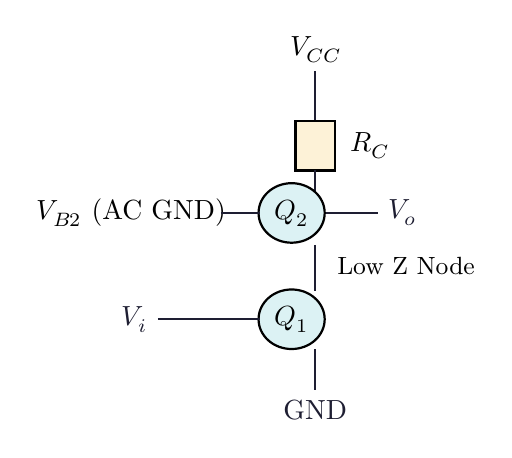
\begin{tikzpicture}[x=1cm,y=0.9cm]
  \node at (2,4.8) {$V_{CC}$};
  \draw[line] (2,4.5)--(2,3.8);
  \draw[thick,fill=hdramber] (1.75,3.1) rectangle (2.25,3.8);
  \node[right=2pt] at (2.25,3.45) {$R_C$};
  \draw[line] (2,3.1)--(2,2.5);
  \draw[line] (2,2.5)--(2.8,2.5) node[right] {$V_o$};

  % Q2 (CB)
  \draw[thick,fill=hdrteal] (1.7,2.5) circle (0.42);
  \node at (1.7,2.5) {$Q_2$};
  \node[left=6pt] at (1.2,2.5) {$V_{B2}$ (AC GND)};
  \draw[line] (0.8,2.5)--(1.3,2.5);

  \draw[line] (2,2.05)--(2,1.4);
  \node[right=3pt] at (2.05,1.75) {\small Low Z Node};

  % Q1 (CE)
  \draw[thick,fill=hdrteal] (1.7,1.0) circle (0.42);
  \node at (1.7,1.0) {$Q_1$};
  \draw[line] (0,1.0)--(1.3,1.0) node[pos=0,left] {$V_i$};
  \draw[line] (2,0.58)--(2,0) node[below] {GND};
\end{tikzpicture}\par
\small Input stage $Q_1$ sees load $R_{in2} \approx 1/g_m \approx 26\,\Omega$, keeping $|A_{v1}| \approx 1$ and suppressing Miller multiplication.
\end{tcolorbox}

\section{Power Amplifiers (Large-Signal Classification)}

\begin{tcolorbox}[defbox, title={Classification of Power Amplifiers by Conduction Angle}]
Power amplifiers are designed to deliver maximum $ac$ power to a low-impedance load (e.g., $4\,\Omega$--$8\,\Omega$ loudspeaker) with minimum harmonic distortion and maximum collector conversion efficiency $\eta = P_{ac} / P_{dc}$.
\end{tcolorbox}

\par\vspace{6pt}\noindent
\begin{tabularx}{\linewidth}{|B{2.2cm}|B{2.6cm}|B{2.7cm}|Y|}
\hline
\textbf{Class} & \textbf{Conduction Angle ($\theta$)} & \textbf{Max Efficiency ($\eta$)} & \textbf{Distortion \& Applications} \\
\hline
\textbf{Class A} & $360^\circ$ (Full cycle) & $25\%$ (Series-fed)\newline $50\%$\newline (Transformer) & Lowest distortion; high quiescent dissipation; audio preamps. \\
\hline
\textbf{Class B} & $180^\circ$ (Half cycle) & $\frac{\pi}{4} \approx 78.5\%$ & Push-pull topology; suffers from \textbf{crossover distortion}. \\
\hline
\textbf{Class AB}& $180^\circ < \theta < 360^\circ$ & $50\%$ to $78.5\%$ & Slight forward bias eliminates crossover distortion; standard audio output stage. \\
\hline
\textbf{Class C} & $\theta < 180^\circ$ ($\sim 120^\circ$) & $> 85\%$ & Extreme non-linearity; tuned LC tank extracts carrier; RF transmitters. \\
\hline
\textbf{Class D} & Switching (PWM) & $\approx 95\%$--$98\%$ & Transistors act as on/off switches; negligible dissipation; modern compact audio/subwoofers. \\
\hline
\end{tabularx}
\par\vspace{12pt}

\subsection{Class B and Class AB Push-Pull Operation}
In a Class B push-pull amplifier, two complementary transistors ($NPN$ and $PNP$) conduct alternately:
\[
\begin{aligned}
P_{dc} &= V_{CC} I_{dc} = V_{CC} \left(\frac{2I_m}{\pi}\right) = \frac{2V_{CC}V_m}{\pi R_L},\\
P_{ac} &= \frac{V_m^2}{2R_L},\\
\eta &= \frac{P_{ac}}{P_{dc}} = \frac{V_m^2 / (2R_L)}{2V_{CC}V_m / (\pi R_L)} = \frac{\pi}{4}\left(\frac{V_m}{V_{CC}}\right).
\end{aligned}
\]
At maximum unclipped swing ($V_m = V_{CC}$), efficiency reaches $\eta_{\max} = \pi/4 \approx 78.5\%$.
\begin{itemize}[leftmargin=1.5em, itemsep=2pt]
  \item \textbf{Crossover Distortion}: Neither transistor conducts when the input voltage is within $\pm 0.7\,\mathrm{V}$ of zero (below the cut-in voltage $V_\gamma$). This creates a dead band in the output waveform.
  \item \textbf{Class AB Remedy}: Biasing diodes or a $V_{BE}$-multiplier circuit provide a small quiescent forward bias voltage ($V_{bias} \approx 2 V_\gamma \approx 1.4\,\mathrm{V}$), maintaining a trickle quiescent current ($I_{CQ}$) that eliminates crossover distortion.
\end{itemize}

\section{Feedback Amplifiers: Topologies and Systematic Analysis}

\begin{tcolorbox}[defbox, title={Feedback Principle and Closed-Loop Gain}]
Negative feedback samples the output signal $X_o$ and feeds back a fraction $X_f = \beta X_o$ in phase opposition to the input signal $X_s$. The error signal applied to the basic amplifier is $X_i = X_s - X_f$.
\[
A_f = \frac{X_o}{X_s} = \frac{A X_i}{X_i + \beta A X_i} = \frac{A}{1 + A\beta}.
\]
Here $A$ is open-loop gain, $\beta$ is feedback factor, $A\beta$ is loop gain, and $(1+A\beta)$ is the \textbf{desensitivity / feedback factor}.
\end{tcolorbox}

\subsection{The Four Basic Feedback Topologies}
Depending on whether the output voltage or current is sampled, and whether the feedback signal is mixed in series (voltage subtraction) or shunt (current subtraction):

\begin{enumerate}[leftmargin=1.5em, itemsep=3pt]
  \item \textbf{Voltage-Series (Series-Shunt) Feedback}: Samples output voltage, mixes feedback voltage in series at input:
  \[
  R_{if} = R_i (1 + A\beta),\qquad R_{of} = \frac{R_o}{1 + A\beta}.
  \]
  \textit{Ideal for Voltage Amplifiers} ($R_{if} \to \infty, R_{of} \to 0$). Example: Non-inverting Op-Amp, Emitter Follower.
  \item \textbf{Current-Series (Series-Series) Feedback}: Samples output current, mixes feedback voltage in series:
  \[
  R_{if} = R_i (1 + A\beta),\qquad R_{of} = R_o (1 + A\beta).
  \]
  \textit{Ideal for Transconductance Amplifiers} ($R_{if} \to \infty, R_{of} \to \infty$). Example: CE amplifier with unbypassed emitter resistor $R_E$.
  \item \textbf{Voltage-Shunt (Shunt-Shunt) Feedback}: Samples output voltage, mixes feedback current in shunt:
  \[
  R_{if} = \frac{R_i}{1 + A\beta},\qquad R_{of} = \frac{R_o}{1 + A\beta}.
  \]
  \textit{Ideal for Transresistance Amplifiers} ($R_{if} \to 0, R_{of} \to 0$). Example: Collector-base feedback resistor amplifier, Inverting Op-Amp.
  \item \textbf{Current-Shunt (Shunt-Series) Feedback}: Samples output current, mixes feedback current in shunt:
  \[
  R_{if} = \frac{R_i}{1 + A\beta},\qquad R_{of} = R_o (1 + A\beta).
  \]
  \textit{Ideal for Current Amplifiers} ($R_{if} \to 0, R_{of} \to \infty$). Example: Two-stage BJT current amplifier with emitter-to-base feedback.
\end{enumerate}

\subsection{Effects of Negative Feedback on Amplifier Performance}
\begin{tcolorbox}[formulabox, title={Quantitative Benefits of Negative Feedback}]
\begin{enumerate}[leftmargin=1.5em, itemsep=2pt]
  \item \textbf{Gain Desensitization}:
  Differentiating $A_f = A/(1+A\beta)$:
  \[
  \frac{dA_f}{A_f} = \frac{1}{1 + A\beta}\left(\frac{dA}{A}\right).
  \]
  Gain stability increases by the factor $(1+A\beta)$.
  \item \textbf{Bandwidth Extension}:
  Upper cutoff increases and lower cutoff decreases:
  \[
  f_{Hf} = f_H (1 + A\beta),\qquad f_{Lf} = \frac{f_L}{1 + A\beta},\qquad \mathrm{BW}_f \approx \mathrm{BW}(1 + A\beta).
  \]
  \item \textbf{Non-Linear Harmonic Distortion Reduction}:
  Harmonic distortion generated within the amplifier is suppressed:
  \[
  D_f = \frac{D}{1 + A\beta}.
  \]
  \item \textbf{Noise Reduction}: Noise generated within the feedback loop is reduced by $(1+A\beta)$. (Noise present at the signal source is amplified equally).
\end{enumerate}
\end{tcolorbox}

\begin{tcolorbox}[examplebox, title={Gain Stabilization and Bandwidth Expansion Calculation}]
An open-loop amplifier has $A = 1000 \pm 100$ ($10\%$ variation), $f_L = 50\,\mathrm{Hz}$, and $f_H = 20\,\mathrm{kHz}$. Design negative feedback with $\beta = 0.049$.
\[
\begin{aligned}
\text{Desensitivity factor:}\quad 1 + A\beta &= 1 + 1000(0.049) = 1 + 49 = 50,\\
\text{Closed-loop gain:}\quad A_f &= \frac{A}{1 + A\beta} = \frac{1000}{50} = 20,\\
\text{Fractional gain variation:}\quad \frac{dA_f}{A_f} &= \frac{1}{50}\left(\frac{dA}{A}\right) = \frac{10\%}{50} = 0.2\%,\\
\text{New bandwidth:}\quad f_{Hf} &= 20\,\mathrm{kHz} \times 50 = 1000\,\mathrm{kHz} = 1\,\mathrm{MHz},\\
f_{Lf} &= 50\,\mathrm{Hz} / 50 = 1\,\mathrm{Hz}.
\end{aligned}
\]
Negative feedback stabilizes gain to within $0.2\%$ and expands bandwidth from $20\,\mathrm{kHz}$ to $1\,\mathrm{MHz}$.
\end{tcolorbox}

\newpage

% ─── Quick Revision Page ───────────────────────────────────────────────────────
\begin{center}
  {\large\bfseries\color{myred} Quick Revision --- Module 2}\\[3pt]
  {\small\color{mydark} Frequency Response, Power Amplifiers and Feedback $|$ EC402}
\end{center}
\noindent{\color{myred}\rule{\linewidth}{1.2pt}}
\vspace{4pt}

\begin{tcolorbox}[formulabox, title={Key Formulas at a Glance}]
\small
\renewcommand{\arraystretch}{1.35}
\setlength{\tabcolsep}{5pt}
\noindent\begin{tabularx}{\linewidth}{B{4.1cm}Y}
Beta Cutoff Frequency ($f_\beta$) & $f_\beta = \frac{1}{2\pi r_{b'e}(C_{b'e}+C_{b'c})} = \frac{1}{2\pi r_\pi (C_\pi + C_\mu)}$ \\[3pt]
Unity-Gain Frequency ($f_T$) & $f_T = h_{fe} f_\beta = \frac{g_m}{2\pi (C_{b'e}+C_{b'c})}$ \\[3pt]
Miller Input Capacitance & $C_{Mi} = C_f(1 + |A_v|)$ \newline $C_{Mo} = C_f(1 + 1/|A_v|) \approx C_f$ \\[3pt]
Multistage Bandwidth Shrink & $f_{H(n)} = f_H \sqrt{2^{1/n}-1}$ \newline $f_{L(n)} = f_L / \sqrt{2^{1/n}-1}$ \\[3pt]
Cascode Miller Capacitance & $C_{M1} = C_{b'c1}(1 + |-1|) = 2C_{b'c1}$ (virtually no Miller multiplication) \\[3pt]
Class B Efficiency ($\eta$) & $\eta = \frac{\pi}{4}\left(\frac{V_m}{V_{CC}}\right)$ \newline $\eta_{\max} = \frac{\pi}{4} \approx 78.5\%$ \\[3pt]
Closed-Loop Feedback Gain & $A_f = \frac{A}{1+A\beta}$ \newline Desensitivity factor $= (1+A\beta)$ \\[3pt]
Feedback Input Resistance & $R_{if} = R_i(1+A\beta)$ (Series) \newline $R_{if} = R_i/(1+A\beta)$ (Shunt) \\[3pt]
Feedback Output Resistance & $R_{of} = R_o/(1+A\beta)$ (Voltage) \newline $R_{of} = R_o(1+A\beta)$ (Current) \\[3pt]
Distortion \& Noise Reduction& $D_f = \frac{D}{1+A\beta}$ \newline $\mathrm{BW}_f = \mathrm{BW}(1+A\beta)$
\end{tabularx}\par
\end{tcolorbox}

\begin{tcolorbox}[defbox, title={One-Line Definitions}, title after break={One-Line Definitions (contd.)}]
\small
\interlinepenalty=10000
\begin{itemize}[leftmargin=1.5em, topsep=2pt, itemsep=4pt]
  \item \textbf{Beta Cutoff Frequency ($f_\beta$)}: The frequency at which the common-emitter short-circuit current gain drops by $3\,\mathrm{dB}$ ($0.707$) from its low-frequency value $h_{fe}$.
  \item \textbf{Unity-Gain Frequency ($f_T$)}: The frequency at which the short-circuit forward current gain of a BJT drops to unity ($0\,\mathrm{dB}$).
  \item \textbf{Miller Effect}: A capacitance between the input and output of an inverting amplifier appears larger at the input. A feedback capacitance $C_f$ contributes $C_f(1+|A_v|)$ when $A_v$ is real and negative.
  \item \textbf{Cascode Amplifier}: A common-emitter stage that feeds a common-base stage. The common-base stage limits the voltage swing at the first collector, reducing Miller multiplication.
  \item \textbf{Cross-Over Distortion}: Distortion near the zero crossing in a Class B push-pull amplifier, where neither output transistor conducts during the handover.
  \item \textbf{Conduction Angle}: The total portion of an input sinusoidal cycle (in degrees or radians) during which the active output device conducts current.
  \item \textbf{Desensitivity}: The factor $1+A\beta$ by which negative feedback reduces the fractional change in closed-loop gain relative to the fractional change in open-loop gain.
  \item \textbf{Voltage-Series Feedback}: A feedback topology that samples output voltage and feeds back a proportional voltage in series opposition, raising input impedance and lowering output impedance.
\end{itemize}
\end{tcolorbox}

\begin{tcolorbox}[exambox, title={Frequently Asked / Viva Questions}]
\begin{enumerate}[topsep=0pt, label=\textbf{Q\arabic*.}, itemsep=5pt]
  \item \Q{What is the physical origin of $C_{b'e}$ and $C_{b'c}$ in the Giacoletto model?}
  $C_{b'e}$ is dominated by the forward-bias emitter diffusion capacitance $C_d$ (caused by minority carrier storage in the base); $C_{b'c}$ is the transition/depletion capacitance of the reverse-biased collector-base junction.

  \item \Q{Why does a Common Emitter amplifier have a much lower high-frequency cutoff than a Common Base amplifier?}
  Because the CE amplifier has high inverting voltage gain, triggering the Miller effect which multiplies $C_{b'c}$ by $(1+|A_v|)$ to create a huge shunt input capacitance; in CB, the base is grounded, completely decoupling input from output.

  \item \Q{How does the Cascode configuration eliminate the Miller effect without sacrificing voltage gain?}
  The input CE transistor drives the low input impedance of the CB stage ($1/g_m$), holding the CE stage voltage gain at $A_{v1} \approx -1$ so its Miller multiplier is only $(1+1)=2$; the CB stage then provides the full voltage gain without any Miller multiplication.

  \item \Q{Why is the maximum theoretical efficiency of a Class B amplifier $78.5\%$ while Class A is only $25\%$?}
  In Class A, DC current flows for the full $360^\circ$ even with zero input signal, causing massive standby dissipation; Class B draws current only for $180^\circ$ in proportion to the signal, with zero standby dissipation under quiescent conditions.

  \item \Q{How is cross-over distortion completely eliminated in audio power amplifiers?}
  By operating in Class AB: placing two forward-biased diodes (or a $V_{BE}$-multiplier circuit) between the bases of the complementary transistors, maintaining a small quiescent trickle bias ($V_{BB} \approx 1.4\,\mathrm{V}$).

  \item \Q{What are the four feedback topologies and their effect on terminal impedances?}
  Voltage-series: $R_i \uparrow, R_o \downarrow$; Current-series: $R_i \uparrow, R_o \uparrow$; Voltage-shunt: $R_i \downarrow, R_o \downarrow$; Current-shunt: $R_i \downarrow, R_o \uparrow$.

  \item \Q{Prove that negative feedback expands amplifier bandwidth.}
  With feedback, $f_{Hf} = f_H(1+A\beta)$ and $f_{Lf} = f_L/(1+A\beta)$. Thus, upper cutoff increases and lower cutoff decreases by the same factor $(1+A\beta)$, expanding total bandwidth while maintaining a constant gain-bandwidth product.

  \item \Q{Why does negative feedback reduce non-linear harmonic distortion?}
  Non-linearities generated within the amplifier produce distortion harmonics that are sampled and fed back out-of-phase to the input, canceling a fraction $(1+A\beta)$ of the internal distortion: $D_f = D/(1+A\beta)$.

  \item \Q{Does negative feedback reduce noise present at the input signal source?}
  No. Negative feedback attenuates internal noise generated inside the amplifier loop by $(1+A\beta)$, but input noise entering with the signal is amplified by the exact same closed-loop gain $A_f$, leaving the input SNR unchanged.

  \item \Q{What happens to the overall bandwidth when $n$ identical amplifier stages are cascaded?}
  Overall bandwidth shrinks significantly: $f_{H(n)} = f_H \sqrt{2^{1/n}-1}$ and $f_{L(n)} = f_L / \sqrt{2^{1/n}-1}$. For two stages ($n=2$), $f_{H(2)} \approx 0.64 f_H$ ($36\%$ bandwidth reduction).
\end{enumerate}
\end{tcolorbox}

\begin{tcolorbox}[tikzbox, title={Summary Comparison of the Four Feedback Topologies}]
\renewcommand{\arraystretch}{1.25}
\setlength{\tabcolsep}{5pt}
\noindent\begin{tabularx}{\linewidth}{|B{3.2cm}|B{2.6cm}|B{2.2cm}|B{2.2cm}|Y|}
\hline
\textbf{Topology} & \textbf{Sampled Quantity} & \textbf{Mixed Quantity} & \textbf{Input / Output Z} & \textbf{Ideal Amplifier Type} \\
\hline
\textbf{Voltage-Series} & Output Voltage ($V_o$) & Voltage in Series ($V_f$) & $R_{in}\uparrow$ / $R_{out}\downarrow$ & Voltage Amplifier ($A_v$) \\
\hline
\textbf{Current-Series} & Output Current ($I_o$) & Voltage in Series ($V_f$) & $R_{in}\uparrow$ / $R_{out}\uparrow$ & Transconductance ($G_m$) \\
\hline
\textbf{Voltage-Shunt}  & Output Voltage ($V_o$) & Current in Shunt ($I_f$) & $R_{in}\downarrow$ / $R_{out}\downarrow$ & Transresistance ($R_m$) \\
\hline
\textbf{Current-Shunt}  & Output Current ($I_o$) & Current in Shunt ($I_f$) & $R_{in}\downarrow$ / $R_{out}\uparrow$ & Current Amplifier ($A_i$) \\
\hline
\end{tabularx}\par
\end{tcolorbox}


% -- Module 3 -----------------------------------------------------------------
\modulestart{3}{Oscillator Principles and the Barkhausen Criterion}

\section{Oscillator Principles and the Barkhausen Criterion}

\begin{tcolorbox}[defbox, title={Oscillator Fundamentals}]
An \textbf{oscillator} is an electronic circuit that converts direct current ($dc$) power from a supply into an alternating current ($ac$) waveform of a predetermined frequency without any external $ac$ input signal. It operates on the principle of \textbf{regenerative (positive) feedback}.
\end{tcolorbox}

\subsection{The Barkhausen Criterion for Sustained Oscillations}
For an amplifier with open-loop gain $A(s)$ and feedback network transfer function $\beta(s)$, the closed-loop transfer function with positive feedback is:
\[
A_f(s) = \frac{A(s)}{1 - A(s)\beta(s)}.
\]
A non-zero output can exist with zero input ($X_s = 0$) only if the denominator vanishes at frequency $\omega_0 = 2\pi f_0$:
\[
1 - A(j\omega_0)\beta(j\omega_0) = 0 \iff A(j\omega_0)\beta(j\omega_0) = 1.
\]

\begin{tcolorbox}[formulabox, title={The Two Barkhausen Conditions}]
For self-sustained oscillations of constant amplitude at frequency $\omega_0$:
\begin{enumerate}[leftmargin=1.5em, itemsep=3pt]
  \item \textbf{Loop Gain Magnitude Condition}: The magnitude of the loop gain must equal unity:
  \[
  |A(j\omega_0)\beta(j\omega_0)| = 1.
  \]
  \textit{Practical Design Rule}: To initiate oscillations from thermal noise, the loop gain must initially be slightly greater than unity ($|A\beta| \ge 1.05$--$1.1$). Non-linear amplitude limiting (clamping, FET/thermistor resistance) subsequently stabilizes $|A\beta| = 1$ in steady state.
  \item \textbf{Phase Condition}: The total phase shift around the feedback loop must be $0^\circ$ or an integer multiple of $360^\circ$:
  \[
  \angle A(j\omega_0)\beta(j\omega_0) = 0^\circ \quad\text{or}\quad 2\pi n \quad (n = 0, 1, 2, \dots).
  \]
  If the active amplifier provides a phase shift of $180^\circ$ (inverting stage), the feedback network must introduce an additional $180^\circ$ phase shift at frequency $f_0$.
\end{enumerate}
\end{tcolorbox}

\section{Audio-Frequency ($RC$) and Radio-Frequency ($LC$) Oscillators}

\subsection{$RC$ Phase Shift Oscillator (Audio Range: $10\,\mathrm{Hz}$--$100\,\mathrm{kHz}$)}
An inverting amplifier ($180^\circ$ phase shift) is cascaded with a three-section high-pass $RC$ ladder network. Each $RC$ section produces an average phase shift of $60^\circ$, providing the required $180^\circ$ feedback phase shift.

\begin{tcolorbox}[formulabox, title={Derivation of $RC$ Phase Shift Oscillator Frequency}]
Applying KVL to the three-mesh ladder network, the feedback transfer function $\beta(s) = V_f(s)/V_o(s)$ (with $\alpha = 1/(sRC)$) is:
\[
\beta(s) = \frac{1}{1 + 6\alpha + 5\alpha^2 + \alpha^3} = \frac{1}{1 - \dfrac{5}{\omega^2 R^2 C^2} - j\left(\dfrac{6}{\omega R C} - \dfrac{1}{\omega^3 R^3 C^3}\right)}.
\]
To satisfy the phase condition $\angle \beta = 180^\circ$, the imaginary part must vanish:
\[
\frac{6}{\omega_0 R C} - \frac{1}{\omega_0^3 R^3 C^3} = 0 \implies \omega_0^2 = \frac{1}{6 R^2 C^2} \implies f_0 = \frac{1}{2\pi R C \sqrt{6}}.
\]
Substituting $\omega_0$ into the real part:
\[
\beta(j\omega_0) = \frac{1}{1 - 5(6)} = -\frac{1}{29}.
\]
To satisfy the loop gain condition $|A_v \beta| \ge 1$, the amplifier voltage gain must satisfy:
\[
|A_v| \ge 29.
\]
For a BJT circuit with collector load $R_C = k R$, the frequency becomes $f_0 = \frac{1}{2\pi R C \sqrt{6 + 4k}}$ and $h_{fe} \ge 44.5 + 23k + 4/k$.
\end{tcolorbox}

\subsection{Wien Bridge Oscillator (Laboratory Standard: $10\,\mathrm{Hz}$--$1\,\mathrm{MHz}$)}
Uses a non-inverting amplifier ($0^\circ$ phase shift) with a series $RC$ and parallel $RC$ lead-lag bridge network:
\[
Z_s = R + \frac{1}{sC} = \frac{sRC + 1}{sC},\qquad
Z_p = R \parallel \frac{1}{sC} = \frac{R}{sRC + 1}.
\]
The feedback transfer function is:
\[
\beta(s) = \frac{Z_p}{Z_s + Z_p} = \frac{sRC}{(sRC)^2 + 3sRC + 1} = \frac{1}{3 + j\left(\omega RC - \dfrac{1}{\omega RC}\right)}.
\]

\begin{tcolorbox}[formulabox, title={Wien Bridge Oscillation Frequency and Gain Condition}]
To make the phase shift zero ($\angle \beta = 0^\circ$), the imaginary term must vanish:
\[
\omega_0 RC - \frac{1}{\omega_0 RC} = 0 \implies \omega_0 = \frac{1}{RC} \implies f_0 = \frac{1}{2\pi RC}.
\]
At resonance $\omega_0$, $\beta(j\omega_0) = 1/3$. The non-inverting amplifier gain $A_v = 1 + R_f/R_1$ must satisfy:
\[
|A_v \beta| \ge 1 \implies A_v \ge 3 \iff \frac{R_f}{R_1} \ge 2.
\]
\end{tcolorbox}

\subsection{$LC$ Resonant Tank Oscillators (RF Range: $100\,\mathrm{kHz}$--$500\,\mathrm{MHz}$)}
A general three-terminal reactive feedback network satisfies $X_1 + X_2 + X_3 = 0$:
\begin{enumerate}[leftmargin=1.5em, itemsep=3pt]
  \item \textbf{Hartley Oscillator}: Uses two inductors ($L_1, L_2$ with mutual inductance $M$) and one tuning capacitor $C$:
  \[
  L_{eq} = L_1 + L_2 + 2M,\qquad
  f_0 = \frac{1}{2\pi \sqrt{L_{eq} C}},\qquad
  A_v \ge \frac{L_1 + M}{L_2 + M}.
  \]
  \item \textbf{Colpitts Oscillator}: Uses two capacitors ($C_1, C_2$) and one inductor $L$:
  \[
  C_{eq} = \frac{C_1 C_2}{C_1 + C_2},\qquad
  f_0 = \frac{1}{2\pi \sqrt{L C_{eq}}},\qquad
  A_v \ge \frac{C_2}{C_1}.
  \]
  \item \textbf{Clapp Oscillator}: Adds a small series capacitor $C_3 \ll C_1, C_2$ in series with $L$:
  \[
  \frac{1}{C_{eq}} = \frac{1}{C_1} + \frac{1}{C_2} + \frac{1}{C_3} \approx \frac{1}{C_3} \implies f_0 \approx \frac{1}{2\pi \sqrt{L C_3}}.
  \]
  \textit{Key Advantage}: Transistor parasitic junction capacitances appear across $C_1$ and $C_2$. Since $C_3 \ll C_1, C_2$, $C_{eq}$ is determined almost exclusively by $C_3$, giving exceptional frequency stability.
  \item \textbf{Crystal Oscillator}: Employs a piezoelectric quartz crystal. Series resonant frequency $f_s = \frac{1}{2\pi\sqrt{L C}}$ (low impedance) and parallel resonant frequency $f_p = \frac{1}{2\pi\sqrt{L [C C_0/(C+C_0)]}}$ (antiresonance, high impedance). Offers $Q$-factors of $10^4$--$10^6$ and frequency stability of $\pm 1\,\mathrm{ppm}$.
\end{enumerate}

\section{Multivibrators: Astable, Monostable and Bistable}

\begin{tcolorbox}[defbox, title={Multivibrator Classification}]
Multivibrators are two-stage cross-coupled non-sinusoidal switching circuits:
\begin{itemize}[leftmargin=1.5em, itemsep=2pt]
  \item \textbf{Astable (Free-Running)}: Zero stable states; toggles continuously between two quasi-stable states, generating a periodic square wave.
  \item \textbf{Monostable (One-Shot)}: One stable state, one quasi-stable state. An external trigger pulse causes a transition to the quasi-stable state for a predetermined duration $T$.
  \item \textbf{Bistable (Flip-Flop)}: Two stable states; requires external trigger pulses to switch between states. Used for digital memory storage.
\end{itemize}
\end{tcolorbox}

\subsection{Astable Multivibrator Waveform Timing}
In a symmetrical cross-coupled BJT circuit with collector resistors $R_C$ and base resistors $R$:
\[
T_1 = R_1 C_1 \ln(2) \approx 0.693 R_1 C_1,\qquad
T_2 = R_2 C_2 \ln(2) \approx 0.693 R_2 C_2.
\]
Total period and oscillation frequency:
\[
T = T_1 + T_2 = 1.386 RC,\qquad f = \frac{1}{T} = \frac{1}{1.386 RC} \approx \frac{0.72}{RC}.
\]

\section{Current Mirrors: Topologies, $V-I$ Curves and Output Resistance}

\begin{tcolorbox}[defbox, title={Current Mirror Concept}]
A \textbf{current mirror} uses a reference current $I_{ref}$ to set an output current $I_o$ in a matched transistor. The output current can equal the reference current or be a fixed multiple of it. A high output resistance helps keep $I_o$ steady as the output voltage changes.
\end{tcolorbox}

\subsection{Basic BJT Current Mirror Analysis}
Consider two matched transistors $Q_1, Q_2$ with $Q_1$ connected as a diode ($V_{CE1} = V_{BE1} = V_{BE2}$):
\[
I_{ref} = \frac{V_{CC} - V_{BE}}{R} = I_{C1} + I_{B1} + I_{B2} = I_{C1} + \frac{2I_C}{\beta}.
\]
Assuming identical matched transistors ($I_{C1} = I_{C2} = I_o$):
\[
I_{ref} = I_o \left(1 + \frac{2}{\beta}\right) \implies I_o = \frac{I_{ref}}{1 + \dfrac{2}{\beta}} \approx I_{ref}\left(1 - \frac{2}{\beta}\right).
\]
\textbf{Finite Output Resistance ($R_o$)}: Due to the Early effect ($V_A$), $I_o$ increases slightly with output voltage $V_{CE2}$:
\[
I_o = I_{ref}\left(1 - \frac{2}{\beta}\right)\left(1 + \frac{V_{CE2} - V_{BE}}{V_A}\right),\qquad R_o = \frac{\partial V_{CE2}}{\partial I_o} \approx r_{o2} = \frac{V_A}{I_o}.
\]
\textbf{Minimum Sustainable Voltage ($V_{ON}$)}: To keep $Q_2$ in the active region, $V_{CE2} \ge V_{CE,\mathrm{sat}} \approx 0.2\,\mathrm{V}$ (or $V_{DS} \ge V_{ov} = V_{GS} - V_{th}$ for MOSFETs). Maximum usable load resistance: $R_{L,\max} = (V_{CC} - V_{ON})/I_o$.

\begin{tcolorbox}[tikzbox, unbreakable, title={Basic, Widlar and Wilson Current Mirror Topologies}]
\centering
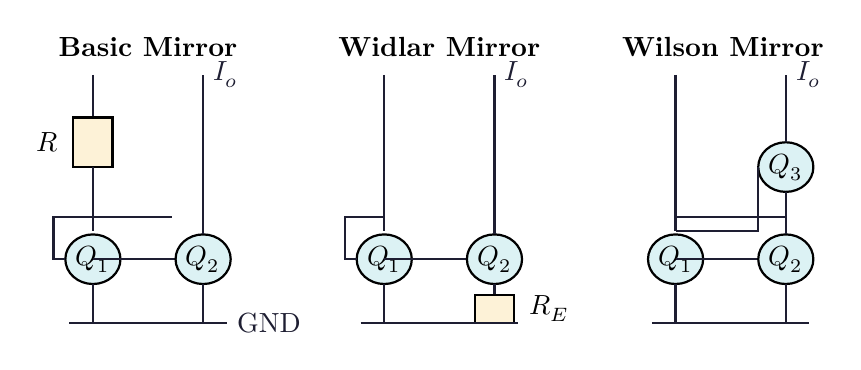
\begin{tikzpicture}[x=1cm,y=0.9cm]
  % Basic Mirror
  \node at (1.5,4.2) {\bfseries Basic Mirror};
  \draw[line] (0.8,3.8)--(0.8,3.2);
  \draw[thick,fill=hdramber] (0.55,2.5) rectangle (1.05,3.2);
  \node[left=2pt] at (0.55,2.85) {$R$};
  \draw[line] (0.8,2.5)--(0.8,1.6);
  % Q1
  \draw[thick,fill=hdrteal] (0.8,1.2) circle (0.35); \node at (0.8,1.2) {$Q_1$};
  % Diode connection
  \draw[line] (0.8,1.8)--(0.3,1.8)--(0.3,1.2)--(0.45,1.2);
  \draw[line] (0.8,1.8)--(1.8,1.8);
  % Base line
  \draw[line] (0.8,1.2)--(2.2,1.2);
  % Q2
  \draw[thick,fill=hdrteal] (2.2,1.2) circle (0.35); \node at (2.2,1.2) {$Q_2$};
  \draw[line] (2.2,1.55)--(2.2,3.8) node[right] {$I_o$};
  \draw[line] (0.8,0.85)--(0.8,0.3);
  \draw[line] (2.2,0.85)--(2.2,0.3);
  \draw[line] (0.5,0.3)--(2.5,0.3) node[right] {GND};

  % Widlar Mirror
  \node at (5.2,4.2) {\bfseries Widlar Mirror};
  \draw[line] (4.5,3.8)--(4.5,1.6);
  \draw[thick,fill=hdrteal] (4.5,1.2) circle (0.35); \node at (4.5,1.2) {$Q_1$};
  \draw[line] (4.5,1.8)--(4.0,1.8)--(4.0,1.2)--(4.15,1.2);
  \draw[line] (4.5,1.2)--(5.9,1.2);
  \draw[thick,fill=hdrteal] (5.9,1.2) circle (0.35); \node at (5.9,1.2) {$Q_2$};
  \draw[line] (5.9,1.55)--(5.9,3.8) node[right] {$I_o$};
  \draw[line] (4.5,0.85)--(4.5,0.3);
  \draw[line] (5.9,0.85)--(5.9,0.7);
  \draw[thick,fill=hdramber] (5.65,0.3) rectangle (6.15,0.7);
  \node[right=2pt] at (6.15,0.5) {$R_E$};
  \draw[line] (4.2,0.3)--(6.2,0.3);

  % Wilson Mirror
  \node at (8.8,4.2) {\bfseries Wilson Mirror};
  \draw[line] (8.2,3.8)--(8.2,1.6);
  \draw[thick,fill=hdrteal] (8.2,1.2) circle (0.35); \node at (8.2,1.2) {$Q_1$};
  \draw[line] (8.2,1.2)--(9.6,1.2);
  \draw[thick,fill=hdrteal] (9.6,1.2) circle (0.35); \node at (9.6,1.2) {$Q_2$};
  \draw[thick,fill=hdrteal] (9.6,2.5) circle (0.35); \node at (9.6,2.5) {$Q_3$};
  \draw[line] (9.6,2.85)--(9.6,3.8) node[right] {$I_o$};
  \draw[line] (9.6,1.55)--(9.6,2.15);
  \draw[line] (8.2,1.6)--(9.25,1.6)--(9.25,2.5)--(9.25,2.5);
  \draw[line] (9.6,1.8)--(8.2,1.8);
  \draw[line] (8.2,0.85)--(8.2,0.3);
  \draw[line] (9.6,0.85)--(9.6,0.3);
  \draw[line] (7.9,0.3)--(9.9,0.3);
\end{tikzpicture}\par
\small Widlar inserts $R_E$ to synthesize small microampere currents; Wilson adds $Q_3$ providing negative feedback that boosts output resistance to $R_o \approx \beta r_o / 2$.
\end{tcolorbox}

\subsection{Advanced Variants: Widlar and Wilson Current Mirrors}
\begin{enumerate}[leftmargin=1.5em, itemsep=3pt]
  \item \textbf{Widlar Current Mirror (Microampere Current Source)}:
  In IC design, generating small bias currents ($I_o \sim 1$--$10\,\mu\mathrm{A}$) using the basic mirror would require enormous resistance: $R = (V_{CC}-V_{BE})/I_{ref} \approx 10\,\mathrm{V}/10\,\mu\mathrm{A} = 1\,\mathrm{M}\Omega$ (consuming huge silicon die area). Widlar inserts an emitter degeneration resistor $R_E$ in $Q_2$:
  \[
  V_{BE1} - V_{BE2} = I_o R_E \implies V_T \ln\left(\frac{I_{ref}}{I_o}\right) = I_o R_E.
  \]
  A reference current of $I_{ref} = 1\,\mathrm{mA}$ yields $I_o = 10\,\mu\mathrm{A}$ with $R_E = \frac{26\,\mathrm{mV}}{10\,\mu\mathrm{A}}\ln(100) \approx 11.9\,\mathrm{k}\Omega$, reducing silicon area by over $98\%$.
  \item \textbf{Wilson Current Mirror}:
  Adds a third transistor $Q_3$. Transistor $Q_3$ samples $I_o$ and applies negative feedback to $Q_1$, which stabilizes $I_o$ against $\beta$ variations:
  \[
  I_o = I_{ref}\left(1 - \frac{2}{\beta^2}\right),\qquad
  R_o \approx \frac{\beta r_o}{2}.
  \]
  Increases output dynamic resistance by factor of $\beta/2$ ($50$--$100\times$), approaching an ideal constant current source.
\end{enumerate}

\newpage

% ─── Quick Revision Page ───────────────────────────────────────────────────────
\begin{center}
  {\large\bfseries\color{myred} Quick Revision --- Module 3}\\[3pt]
  {\small\color{mydark} Oscillators, Multivibrators and Current Mirrors $|$ EC402}
\end{center}
\noindent{\color{myred}\rule{\linewidth}{1.2pt}}
\vspace{4pt}

\begin{tcolorbox}[formulabox, title={Key Formulas at a Glance}]
\small
\renewcommand{\arraystretch}{1.35}
\setlength{\tabcolsep}{5pt}
\noindent\begin{tabularx}{\linewidth}{B{4.1cm}Y}
Barkhausen Criterion & $|A\beta| > 1$ at start-up; $|A\beta| = 1$ at steady state \newline $\angle A\beta = 360^\circ n$, $n \in \mathbb{Z}$ \\[3pt]
$RC$ Phase Shift Oscillator & $f_0 = \frac{1}{2\pi RC\sqrt{6}}$ \newline $|A_v| \ge 29$ (Op-Amp / FET) \\[3pt]
Wien Bridge Oscillator & $f_0 = \frac{1}{2\pi RC}$ \newline $A_v \ge 3 \iff R_f \ge 2R_1$ \\[3pt]
Hartley Oscillator & $f_0 = \frac{1}{2\pi \sqrt{L_{eq}C}}$ where $L_{eq} = L_1 + L_2 + 2M$ \\[3pt]
Colpitts Oscillator & $f_0 = \frac{1}{2\pi \sqrt{L C_{eq}}}$ where $C_{eq} = \frac{C_1 C_2}{C_1 + C_2}$ \\[3pt]
Clapp Oscillator & $f_0 \approx \frac{1}{2\pi \sqrt{L C_3}}$ (where $C_3 \ll C_1, C_2$) \\[3pt]
Astable Multivibrator Period & $T = T_1 + T_2 = 0.693(R_1 C_1 + R_2 C_2)$ \newline $T = 1.386 RC$ for equal $R$ and $C$ \\[3pt]
Basic Current Mirror Ratio & $I_o = \frac{I_{ref}}{1 + 2/\beta} \approx I_{ref}\left(1 - \frac{2}{\beta}\right)$ \\[3pt]
Widlar Mirror Equation & $I_o R_E = V_T \ln\left(\frac{I_{ref}}{I_o}\right)$ \\[3pt]
Wilson Output Resistance & $R_o \approx \frac{\beta r_o}{2}$ (boosted by $\beta/2$)
\end{tabularx}\par
\end{tcolorbox}

\begin{tcolorbox}[defbox, title={One-Line Definitions}, title after break={One-Line Definitions (contd.)}]
\small
\interlinepenalty=10000
\begin{itemize}[leftmargin=1.5em, topsep=2pt, itemsep=4pt]
  \item \textbf{Barkhausen Criterion}: The mathematical condition requiring loop gain magnitude $|A\beta|=1$ and loop phase shift $\angle A\beta = 0^\circ$ or $360^\circ$ for sustained sinusoidal oscillation.
  \item \textbf{Lead-Lag Network}: A series-parallel $RC$ feedback network used in the Wien bridge. For equal resistor and capacitor pairs, it gives zero phase shift and a feedback fraction of $1/3$ at $f_0=1/(2\pi RC)$.
  \item \textbf{Piezoelectric Effect}: The generation of an electrical charge across the faces of a crystal when subjected to mechanical stress, and vice versa.
  \item \textbf{Astable Multivibrator}: A switching circuit with no stable state. It switches repeatedly between two temporary states and produces a periodic output without a trigger.
  \item \textbf{Current Mirror}: A circuit that uses a reference current to set an output current, usually to the same value or to a fixed multiple of it.
  \item \textbf{Widlar Current Source}: A BJT current mirror with a resistor in the output transistor's emitter. The resistor makes the output current much smaller than the reference current.
  \item \textbf{Wilson Current Source}: A three-transistor current mirror that uses negative feedback to reduce current error caused by finite $\beta$ and increase output resistance.
  \item \textbf{Compliance Voltage ($V_{ON}$)}: The minimum output voltage a current mirror needs to maintain its set current.
\end{itemize}
\end{tcolorbox}

\begin{tcolorbox}[exambox, title={Frequently Asked / Viva Questions}]
\begin{enumerate}[topsep=0pt, label=\textbf{Q\arabic*.}, itemsep=5pt]
  \item \Q{State the Barkhausen criterion for sustained oscillations.}
  The loop gain magnitude must be unity ($|A\beta| = 1$), and the total phase shift around the closed loop must be $0^\circ$ or an integer multiple of $360^\circ$ ($\angle A\beta = 2\pi n$).

  \item \Q{Why does an $RC$ phase shift oscillator require a minimum amplifier gain of 29?}
  Because at the resonant frequency $f_0 = 1/(2\pi RC\sqrt{6})$, the three-mesh $RC$ ladder network attenuates the signal by exactly $\beta = 1/29$; thus $|A_v| \ge 29$ is strictly required to satisfy $|A_v\beta| \ge 1$.

  \item \Q{Why are $RC$ oscillators preferred at audio frequencies while $LC$ oscillators are used at RF?}
  At audio frequencies ($10\,\mathrm{Hz}$--$20\,\mathrm{kHz}$), $LC$ tank inductors and capacitors become prohibitively bulky and lossy; at RF ($> 1\,\mathrm{MHz}$), $RC$ phase-shift resistors become too small and stray capacitances disrupt phase accuracy.

  \item \Q{What makes the Clapp oscillator more stable than the Colpitts oscillator?}
  The Clapp oscillator places a small capacitor $C_3 \ll C_1, C_2$ in series with the inductor; since $C_{eq} \approx C_3$, the resonant frequency is insulated from transistor junction capacitances appearing across $C_1$ and $C_2$.

  \item \Q{Why does a quartz crystal exhibit two resonant frequencies?}
  Due to its physical mass and elasticity, its equivalent electrical circuit consists of a series $L$-$C$-$R$ motional arm in parallel with electrode mounting capacitance $C_0$, creating series resonance $f_s$ and parallel antiresonance $f_p$.

  \item \Q{What is the duty cycle of a symmetrical astable multivibrator?}
  $50\%$, because $R_1=R_2$ and $C_1=C_2$, meaning $T_1 = 0.693 RC = T_2$ and duty cycle $= T_1/(T_1+T_2) = 0.5$.

  \item \Q{Why is a Widlar current mirror essential in analog integrated circuit design?}
  In ICs, fabricating mega-ohm resistors to generate microampere currents requires massive silicon die area; Widlar's emitter resistor $R_E$ achieves microampere currents using small, area-efficient resistances ($\sim 10\,\mathrm{k}\Omega$).

  \item \Q{How does the Wilson current mirror improve upon the basic current mirror?}
  The additional transistor $Q_3$ provides internal negative feedback that reduces $\beta$-error from $2/\beta$ down to $2/\beta^2$ and boosts the output resistance by $\beta/2$, reaching several mega-ohms.

  \item \Q{What determines the maximum usable load resistance of a current mirror?}
  The supply voltage and the compliance voltage $V_{ON}$: $R_{L,\max} = (V_{CC} - V_{ON}) / I_o$. If $R_L$ exceeds this, the output transistor drops into saturation, collapsing current regulation.

  \item \Q{How do you prevent frequency drift in Wien bridge oscillators?}
  By incorporating negative-temperature-coefficient thermistors or a JFET voltage-controlled resistor in the negative feedback arm ($R_1$), automatically adjusting amplifier gain to exactly $A_v = 3$.
\end{enumerate}
\end{tcolorbox}

\begin{tcolorbox}[tikzbox, title={Summary Comparison of RF and Audio Oscillators}]
\renewcommand{\arraystretch}{1.25}
\setlength{\tabcolsep}{5pt}
\noindent\begin{tabularx}{\linewidth}{|B{3.2cm}|B{3.25cm}|B{2.2cm}|Y|}
\hline
\textbf{Oscillator Type} & \textbf{Frequency Range} & \textbf{Active Gain Req.} & \textbf{Distinguishing Feature} \\
\hline
\textbf{$RC$ Phase Shift}& $10\,\mathrm{Hz}$ to\newline $100\,\mathrm{kHz}$ (Audio) & $|A_v| \ge 29$ & 3-stage $RC$ ladder ($180^\circ$ phase shift) \\
\hline
\textbf{Wien Bridge}     & $10\,\mathrm{Hz}$ to\newline $1\,\mathrm{MHz}$ (Audio/Lab)& $A_v \ge 3$ & Lead-lag network ($0^\circ$ phase shift), low distortion \\
\hline
\textbf{Hartley}         & $100\,\mathrm{kHz}$ to\newline $100\,\mathrm{MHz}$ (RF)  & $A_v \ge L_1/L_2$ & Center-tapped inductor tank \\
\hline
\textbf{Colpitts}        & $1\,\mathrm{MHz}$ to\newline $500\,\mathrm{MHz}$ (RF)    & $A_v \ge C_2/C_1$ & Split-capacitor tank, excellent high-frequency performance \\
\hline
\textbf{Quartz Crystal}  & $10\,\mathrm{kHz}$ to\newline $100\,\mathrm{MHz}$ (Fixed) & Minimal & Highest frequency stability ($Q \approx 10^5$, $\pm 1\,\mathrm{ppm}$) \\
\hline
\end{tabularx}\par
\end{tcolorbox}


% -- Module 4 -----------------------------------------------------------------
\modulestart{4}{BJT Differential Amplifier}

\section{BJT Differential Amplifier}

\begin{tcolorbox}[defbox, title={Definition: Differential Amplifier}]
A \textbf{Differential Amplifier} is a direct-coupled circuit consisting of two matched transistors configured to amplify the algebraic difference between two input signals while attenuating any signal common to both inputs. It forms the essential input stage of operational amplifiers and linear integrated circuits.
\end{tcolorbox}

\subsection{Basic Architecture and Principle of Operation}
The basic emitter-coupled differential amplifier consists of two matched transistors ($Q_1, Q_2$), identical collector resistors $R_{C1} = R_{C2} = R_C$, and an emitter resistance $R_E$ (or an active constant current source $I_{EE}$) connected to negative supply $-V_{EE}$.

\begin{tcolorbox}[tikzbox, title={BJT Emitter-Coupled Differential Pair Architecture}]
\centering
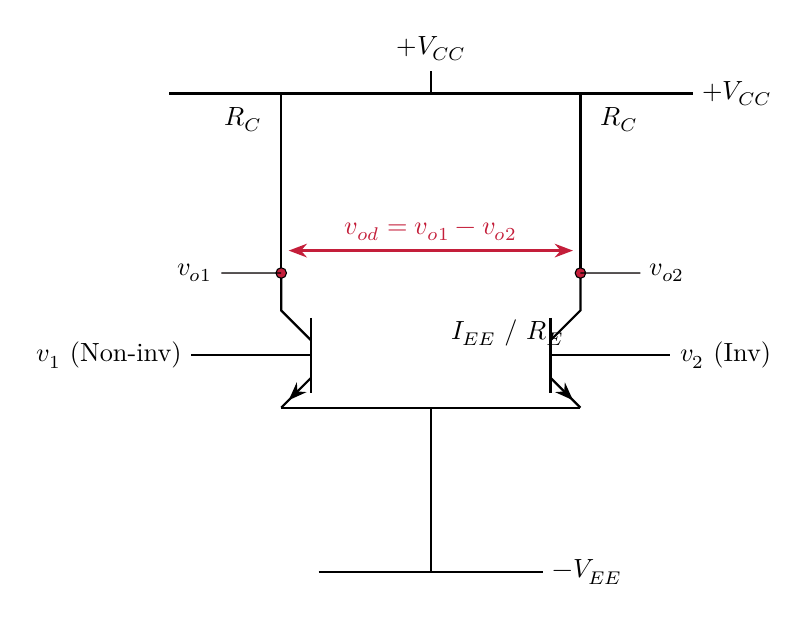
\begin{tikzpicture}[scale=0.95, transform shape]
  % VCC rail
  \draw[thick] (-3.5, 3.2) -- (3.5, 3.2) node[right] {$+V_{CC}$};
  \draw[thick] (0, 3.2) -- (0, 3.5) node[above] {$+V_{CC}$};

  % Resistors RC1, RC2
  \draw[thick] (-2, 3.2) -- (-2, 2.5) to[rectangle, draw=myteal, fill=hdrteal, minimum width=0.6cm, minimum height=1cm] (-2, 1.5) node[midway, left=4pt] {$R_C$} -- (-2, 0.8);
  \draw[thick] (2, 3.2) -- (2, 2.5) to[rectangle, draw=myteal, fill=hdrteal, minimum width=0.6cm, minimum height=1cm] (2, 1.5) node[midway, right=4pt] {$R_C$} -- (2, 0.8);

  % Transistors Q1 and Q2
  \draw[thick] (-2, 0.8) -- (-2, 0.3) -- (-1.6, -0.1); % Collector Q1
  \draw[thick] (-1.6, -0.6) -- (-2, -1.0); % Emitter Q1
  \draw[thick, -Stealth] (-1.8, -0.8) -- (-1.9, -0.9);
  \draw[thick] (-1.6, 0.2) -- (-1.6, -0.8); % Base bar Q1
  \draw[thick] (-1.6, -0.3) -- (-3.2, -0.3) node[left] {$v_1$ (Non-inv)};

  \draw[thick] (2, 0.8) -- (2, 0.3) -- (1.6, -0.1); % Collector Q2
  \draw[thick] (1.6, -0.6) -- (2, -1.0); % Emitter Q2
  \draw[thick, -Stealth] (1.8, -0.8) -- (1.9, -0.9);
  \draw[thick] (1.6, 0.2) -- (1.6, -0.8); % Base bar Q2
  \draw[thick] (1.6, -0.3) -- (3.2, -0.3) node[right] {$v_2$ (Inv)};

  % Common Emitter connection
  \draw[thick] (-2, -1.0) -- (0, -1.0) -- (2, -1.0);
  \draw[thick] (0, -1.0) -- (0, -1.6);

  % Tail current source / RE
  \draw[thick] (0, -1.6) to[rectangle, draw=myamber, fill=hdramber, minimum width=0.7cm, minimum height=1.1cm] (0, -2.7) node[midway, right=4pt] {$I_{EE}$ / $R_E$} -- (0, -3.2);
  \draw[thick] (-1.5, -3.2) -- (1.5, -3.2) node[right] {$-V_{EE}$};

  % Output nodes
  \draw[fill=myred] (-2, 0.8) circle (2pt) -- (-2.8, 0.8) node[left] {$v_{o1}$};
  \draw[fill=myred] (2, 0.8) circle (2pt) -- (2.8, 0.8) node[right] {$v_{o2}$};
  \draw[thick, Stealth-Stealth, color=myred] (-1.9, 1.1) -- (1.9, 1.1) node[midway, above] {$v_{od} = v_{o1} - v_{o2}$};
\end{tikzpicture}
\end{tcolorbox}

\subsection{Large-Signal Transfer Characteristics}
Assuming active region operation where $I_C \approx I_E = I_S e^{V_{BE}/V_T}$:
\begin{align}
  v_1 - v_2 &= v_{id} = V_{BE1} - V_{BE2} = V_T \ln\left(\frac{I_{C1}}{I_{C2}}\right) \\
  \frac{I_{C1}}{I_{C2}} &= e^{v_{id}/V_T}
\end{align}
Since $I_{C1} + I_{C2} = I_{EE}$ (neglecting base currents):
\begin{tcolorbox}[formulabox, title={Large-Signal Differential Collector Currents}]
\begin{equation}
  I_{C1} = \frac{I_{EE}}{1 + e^{-v_{id}/V_T}}, \qquad I_{C2} = \frac{I_{EE}}{1 + e^{v_{id}/V_T}}
\end{equation}
The output differential voltage is:
\begin{equation}
  v_{od} = v_{o1} - v_{o2} = -(I_{C1} - I_{C2})R_C = -I_{EE} R_C \tanh\left(\frac{v_{id}}{2V_T}\right)
\end{equation}
\end{tcolorbox}
\textbf{Linear Range}: For small inputs $|v_{id}| < 2V_T \approx 50\text{ mV}$, $\tanh(x) \approx x$. When $|v_{id}| \ge 4V_T \approx 100\text{ mV}$, current completely steers into one transistor, causing hard saturation/clipping.

\subsection{Small-Signal Half-Circuit Analysis}
Any pair of arbitrary input voltages $v_1, v_2$ can be decomposed into:
\begin{equation}
  v_{id} = v_1 - v_2 \quad (\text{Differential Mode}), \qquad v_{icm} = \frac{v_1 + v_2}{2} \quad (\text{Common Mode})
\end{equation}
such that $v_1 = v_{icm} + \frac{v_{id}}{2}$ and $v_2 = v_{icm} - \frac{v_{id}}{2}$.

\subsubsection{Differential-Mode Half Circuit}
When $v_1 = +v_{id}/2$ and $v_2 = -v_{id}/2$, the circuit exhibits anti-symmetry. The common emitter node potential remains constant at $0\text{ V}$ (virtual ground for differential signals). The tail impedance $R_E$ carries zero signal current:
\begin{tcolorbox}[formulabox, title={Differential Gain ($A_d$) \& Input Impedance ($R_{id}$)}]
\begin{equation}
  A_d = \frac{v_{o1} - v_{o2}}{v_1 - v_2} = -g_m R_C = -\frac{I_{EE} R_C}{2 V_T}
\end{equation}
For single-ended output ($v_o = v_{o1}$):
\begin{equation}
  A_{d,\text{single}} = -\frac{1}{2} g_m R_C
\end{equation}
Differential input resistance:
\begin{equation}
  R_{id} = 2 r_\pi = 2\,\frac{\beta}{g_m} = 4\,\frac{\beta V_T}{I_{EE}}
\end{equation}
\end{tcolorbox}

\subsubsection{Common-Mode Half Circuit}
When $v_1 = v_2 = v_{icm}$, both halves conduct equally in parallel. The tail resistor $R_E$ splits into two parallel resistors of value $2R_E$:
\begin{tcolorbox}[formulabox, title={Common-Mode Gain ($A_c$) \& Input Impedance ($R_{icm}$)}]
\begin{equation}
  A_c = \frac{v_{ocm}}{v_{icm}} = -\frac{g_m R_C}{1 + 2 g_m R_E} \approx -\frac{R_C}{2 R_E} \quad (\text{for } 2g_m R_E \gg 1)
\end{equation}
Common-mode input resistance:
\begin{equation}
  R_{icm} = r_\pi + 2(1+\beta)R_E \approx 2\beta R_E
\end{equation}
\end{tcolorbox}

\subsection{Common-Mode Rejection Ratio (CMRR)}
\begin{tcolorbox}[defbox, title={Common Mode Rejection Ratio}]
\textbf{CMRR} measures the ability of a differential amplifier to reject common-mode noise and amplify only the differential signal:
\begin{equation}
  \text{CMRR} = \left|\frac{A_d}{A_c}\right| = \frac{g_m R_C}{\frac{g_m R_C}{1 + 2g_m R_E}} = 1 + 2g_m R_E \approx 2 g_m R_E = \frac{I_{EE} R_E}{V_T}
\end{equation}
Expressed in decibels:
\begin{equation}
  \text{CMRR}_{\text{dB}} = 20 \log_{10}\left|\frac{A_d}{A_c}\right|
\end{equation}
\end{tcolorbox}
\textbf{Design Implication}: To maximize CMRR, $R_E$ must be made arbitrarily large. In modern IC design, $R_E$ is replaced by an active BJT/MOSFET current mirror, providing incremental output resistance $r_o$ in the megaohm range, pushing CMRR well above $100\text{ dB}$.

\subsection{Input Common-Mode Range (ICMR)}
\begin{tcolorbox}[formulabox, title={Input Common-Mode Range Boundaries}]
$\text{ICMR}$ is the allowable range of common-mode input voltage $v_{icm}$ for which all transistors remain in the active region:
\begin{align}
  V_{icm,\max} &= V_{CC} - I_C R_C + V_{BE} = V_{CC} - \frac{I_{EE} R_C}{2} + 0.7\text{ V} \\
  V_{icm,\min} &= -V_{EE} + V_{CS} + V_{BE}
\end{align}
where $V_{CS}$ is the minimum compliance voltage required across the tail current source to avoid saturation ($\approx 0.3\text{ V}$ for BJT, $V_{ov}$ for MOSFET).
\end{tcolorbox}

% ─── Section 2: Operational Amplifiers ─────────────────────────────────────────
\section{Operational Amplifier (Op-Amp) Fundamentals}

\begin{tcolorbox}[defbox, title={Definition: Operational Amplifier}]
An \textbf{Operational Amplifier (Op-Amp)} is a direct-coupled, high-gain integrated voltage amplifier with differential inputs and single-ended output, designed to perform linear and non-linear mathematical operations via negative and positive feedback networks.
\end{tcolorbox}

\subsection{Internal Architecture: 4-Stage Block Diagram}
\begin{tcolorbox}[tikzbox, title={Internal Block Diagram of Modern IC Op-Amp}]
\centering
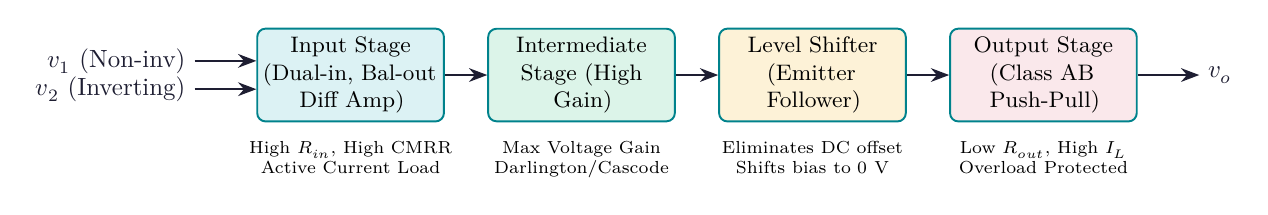
\begin{tikzpicture}[scale=0.9, transform shape, node distance=0.6cm]
  \node[block, fill=hdrteal] (in) {Input Stage\\(Dual-in, Bal-out Diff Amp)};
  \node[block, right=of in, fill=hdrgreen] (inter) {Intermediate\\Stage (High Gain)};
  \node[block, right=of inter, fill=hdramber] (level) {Level Shifter\\(Emitter Follower)};
  \node[block, right=of level, fill=hdrred] (out) {Output Stage\\(Class AB Push-Pull)};

  \draw[arrow] (-2.2, 0.2) node[left] {$v_1$ (Non-inv)} -- (in.west |- 0, 0.2);
  \draw[arrow] (-2.2, -0.2) node[left] {$v_2$ (Inverting)} -- (in.west |- 0, -0.2);
  \draw[arrow] (in) -- (inter);
  \draw[arrow] (inter) -- (level);
  \draw[arrow] (level) -- (out);
  \draw[arrow] (out) -- ++(2.2, 0) node[right] {$v_o$};

  \node[below=0.15cm of in, font=\scriptsize, align=center] {High $R_{in}$, High CMRR\\Active Current Load};
  \node[below=0.15cm of inter, font=\scriptsize, align=center] {Max Voltage Gain\\Darlington/Cascode};
  \node[below=0.15cm of level, font=\scriptsize, align=center] {Eliminates DC offset\\Shifts bias to $0\text{ V}$};
  \node[below=0.15cm of out, font=\scriptsize, align=center] {Low $R_{out}$, High $I_L$\\Overload Protected};
\end{tikzpicture}
\end{tcolorbox}

\subsection{Ideal vs. Practical Op-Amp Characteristics (IC 741)}
\par\vspace{6pt}\noindent
\begin{tabularx}{\linewidth}{|B{3.4cm}|Y|Y|B{3.2cm}|}
\hline
\textbf{Parameter} & \textbf{Ideal Value} & \textbf{Typical IC 741} & \textbf{Significance} \\
\hline
Open-Loop Voltage Gain ($A_{OL}$) & $\infty$ & $2 \times 10^5$ ($106\text{ dB}$) & Eliminates gain error \\
Input Resistance ($R_{in}$) & $\infty$ & $2\text{ M}\Omega$ (FET: $> 10^{12}\Omega$) & Eliminates source loading \\
Output Resistance ($R_{out}$) & $0\,\Omega$ & $75\,\Omega$ & Zero loading by load $R_L$ \\
Bandwidth ($\text{BW}$) & $\infty$ & $1\text{ MHz}$ (Unity GBW) & Constant gain across frequency \\
CMRR & $\infty$ & $90\text{ dB}$ & Rejects common-mode noise \\
Slew Rate ($\text{SR}$) & $\infty$ & $0.5\text{ V}/\mu\text{s}$ & Maximum rate of output swing \\
Input Offset Voltage ($V_{ios}$) & $0\text{ V}$ & $2\text{ mV}$ & DC voltage mismatch at input \\
Input Bias Current ($I_B$) & $0\text{ A}$ & $80\text{ nA}$ & Average DC base currents \\
Input Offset Current ($I_{ios}$) & $0\text{ A}$ & $20\text{ nA}$ & Difference between base currents \\
\hline
\end{tabularx}
\vspace{12pt}

\subsection{Slew Rate and Full-Power Bandwidth}
\begin{tcolorbox}[formulabox, title={Slew Rate and Maximum Frequency Formulation}]
\textbf{Slew Rate (SR)} is the maximum rate of change of output voltage that the op-amp can deliver under large-signal step excitation, limited by the charging of internal compensation capacitor $C_c$:
\begin{equation}
  \text{SR} = \left.\frac{dv_o}{dt}\right|_{\max} = \frac{I_{EE}}{C_c} \quad [\text{V}/\mu\text{s}]
\end{equation}
For an undistorted output sinusoid $v_o(t) = V_m \sin(2\pi f t)$:
\begin{equation}
  \left.\frac{dv_o}{dt}\right|_{\max} = 2\pi f V_m \le \text{SR} \implies f_{\max} = \frac{\text{SR}}{2\pi V_m}
\end{equation}
where $f_{\max}$ is the \textbf{Full-Power Bandwidth}. If input frequency exceeds $f_{\max}$, the output degenerates from a sine wave into a slew-limited triangular wave.
\end{tcolorbox}

\subsection{Basic Inverting and Non-Inverting Configurations}

\begin{tcolorbox}[tikzbox, title={Fundamental Inverting and Non-Inverting Op-Amp Topologies}]
\centering
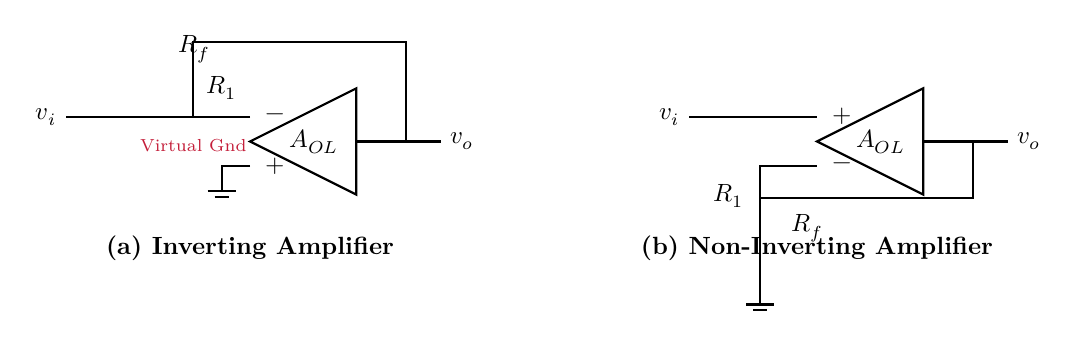
\begin{tikzpicture}[scale=0.9, transform shape]
  % Inverting Amplifier
  \begin{scope}[shift={(-4.2,0)}]
    \draw[thick] (0, 0) -- (1.5, 0.75) -- (1.5, -0.75) -- cycle; % Opamp triangle
    \node at (0.35, 0.35) {$-$};
    \node at (0.35, -0.35) {$+$};
    \node at (0.9, 0) {$A_{OL}$};

    % Inputs
    \draw[thick] (0, 0.35) -- (-0.8, 0.35) to[rectangle, draw=myteal, fill=hdrteal, minimum width=0.8cm, minimum height=0.4cm] (-1.8, 0.35) node[midway, above=3pt] {$R_1$} -- (-2.6, 0.35) node[left] {$v_i$};
    \draw[thick] (0, -0.35) -- (-0.4, -0.35) -- (-0.4, -0.7);
    \draw[thick] (-0.6, -0.7) -- (-0.2, -0.7);
    \draw[thick] (-0.5, -0.78) -- (-0.3, -0.78);

    % Feedback Rf
    \draw[thick] (-0.8, 0.35) -- (-0.8, 1.4) to[rectangle, draw=myteal, fill=hdrteal, minimum width=0.8cm, minimum height=0.4cm] (0.8, 1.4) node[midway, above=3pt] {$R_f$} -- (2.2, 1.4) -- (2.2, 0);

    % Output
    \draw[thick] (1.5, 0) -- (2.7, 0) node[right] {$v_o$};
    \node at (-0.8, 0.15) [below, font=\scriptsize, color=myred] {Virtual Gnd};
    \node at (0, -1.5) [font=\bfseries] {(a) Inverting Amplifier};
  \end{scope}

  % Non-Inverting Amplifier
  \begin{scope}[shift={(3.8,0)}]
    \draw[thick] (0, 0) -- (1.5, 0.75) -- (1.5, -0.75) -- cycle;
    \node at (0.35, 0.35) {$+$};
    \node at (0.35, -0.35) {$-$};
    \node at (0.9, 0) {$A_{OL}$};

    % Input to Non-inv
    \draw[thick] (0, 0.35) -- (-1.8, 0.35) node[left] {$v_i$};

    % Feedback to Inv
    \draw[thick] (0, -0.35) -- (-0.8, -0.35) -- (-0.8, -1.2) to[rectangle, draw=myteal, fill=hdrteal, minimum width=0.4cm, minimum height=0.8cm] (-0.8, -2.0) node[midway, left=3pt] {$R_1$} -- (-0.8, -2.3);
    \draw[thick] (-1.0, -2.3) -- (-0.6, -2.3);
    \draw[thick] (-0.9, -2.38) -- (-0.7, -2.38);

    \draw[thick] (-0.8, -0.35) -- (-0.8, -0.8) -- (0.5, -0.8) to[rectangle, draw=myteal, fill=hdrteal, minimum width=0.8cm, minimum height=0.4cm] (1.5, -0.8) node[midway, below=3pt] {$R_f$} -- (2.2, -0.8) -- (2.2, 0);

    % Output
    \draw[thick] (1.5, 0) -- (2.7, 0) node[right] {$v_o$};
    \node at (0, -1.5) [font=\bfseries] {(b) Non-Inverting Amplifier};
  \end{scope}
\end{tikzpicture}
\end{tcolorbox}

\begin{tcolorbox}[formulabox, title={Inverting \& Non-Inverting Gain Derivations}]
\textbf{Inverting Configuration}:
By virtual ground ($v_- = v_+ = 0\text{ V}$) and $i_- = 0$:
\begin{equation}
  \frac{v_i - 0}{R_1} + \frac{v_o - 0}{R_f} = 0 \implies A_v = \frac{v_o}{v_i} = -\frac{R_f}{R_1}, \qquad R_{in} = R_1
\end{equation}
\textbf{Non-Inverting Configuration}:
By virtual short ($v_- = v_+ = v_i$) and voltage divider across feedback network:
\begin{equation}
  v_- = v_o \left(\frac{R_1}{R_1 + R_f}\right) = v_i \implies A_v = \frac{v_o}{v_i} = 1 + \frac{R_f}{R_1}, \qquad R_{in} \to \infty
\end{equation}
\textbf{Voltage Follower (Buffer)}: When $R_f = 0$ and $R_1 \to \infty$, $A_v = 1$, $R_{in} \approx \infty$, $R_{out} \approx 0$.
\end{tcolorbox}

% ─── Section 3: Op-Amp Applications ───────────────────────────────────────────
\section{Linear and Non-Linear Op-Amp Applications}

\subsection{Summing Amplifier}
An inverting adder sums multiple weighted input voltages at the virtual ground node:
\begin{equation}
  v_o = -\left(\frac{R_f}{R_1} v_1 + \frac{R_f}{R_2} v_2 + \frac{R_f}{R_3} v_3\right)
\end{equation}
If $R_1 = R_2 = R_3 = R$, then $v_o = -\frac{R_f}{R}(v_1 + v_2 + v_3)$. When $R_f = R/3$, the circuit acts as an analog averager.

\subsection{Three Op-Amp Instrumentation Amplifier}
\begin{tcolorbox}[defbox, title={Three Op-Amp Instrumentation Amplifier}]
The standard 3-op-amp instrumentation amplifier provides ultra-high differential input impedance, high CMRR, and user-variable gain controlled by a single resistor $R_G$.
\end{tcolorbox}

\begin{tcolorbox}[tikzbox, title={Schematic of 3-Op-Amp Instrumentation Amplifier}]
\centering
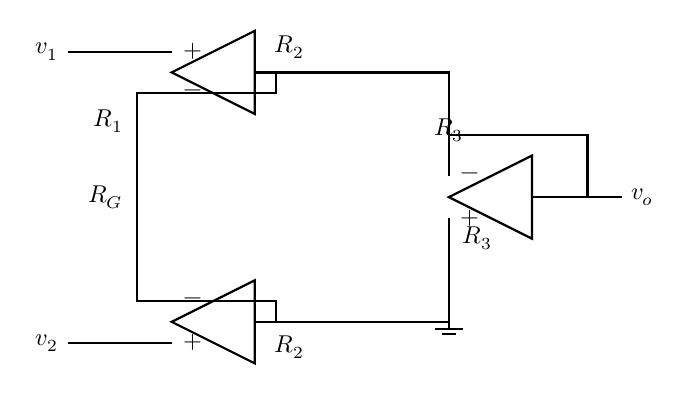
\begin{tikzpicture}[scale=0.88, transform shape]
  % Input Opamp A1
  \draw[thick] (0, 1.8) -- (1.2, 2.4) -- (1.2, 1.2) -- cycle;
  \node at (0.3, 2.1) {$+$}; \node at (0.3, 1.5) {$-$};
  \draw[thick] (0, 2.1) -- (-1.5, 2.1) node[left] {$v_1$};

  % Input Opamp A2
  \draw[thick] (0, -1.8) -- (1.2, -1.2) -- (1.2, -2.4) -- cycle;
  \node at (0.3, -2.1) {$+$}; \node at (0.3, -1.5) {$-$};
  \draw[thick] (0, -2.1) -- (-1.5, -2.1) node[left] {$v_2$};

  % Resistors R1, RG, R1
  \draw[thick] (0, 1.5) -- (-0.5, 1.5) -- (-0.5, 0.7) to[rectangle, draw=myteal, fill=hdrteal, minimum width=0.4cm, minimum height=0.7cm] (-0.5, 0.2) node[midway, left=2pt] {$R_1$} -- (-0.5, -0.2) to[rectangle, draw=myred, fill=hdrred, minimum width=0.4cm, minimum height=0.7cm] (-0.5, -0.7) node[midway, left=2pt] {$R_G$} -- (-0.5, -1.5) -- (0, -1.5);
  \draw[thick] (-0.5, 1.5) -- (1.5, 1.5) -- (1.5, 1.8);
  \draw[thick] (-0.5, -1.5) -- (1.5, -1.5) -- (1.5, -1.8);

  % Output Opamp A3
  \draw[thick] (4, 0) -- (5.2, 0.6) -- (5.2, -0.6) -- cycle;
  \node at (4.3, 0.3) {$-$}; \node at (4.3, -0.3) {$+$};

  % Resistors R2, R3
  \draw[thick] (1.2, 1.8) -- (2.2, 1.8) to[rectangle, draw=myteal, fill=hdrteal, minimum width=0.8cm, minimum height=0.4cm] (3.2, 1.8) node[midway, above=2pt] {$R_2$} -- (4, 1.8) -- (4, 0.3);
  \draw[thick] (1.2, -1.8) -- (2.2, -1.8) to[rectangle, draw=myteal, fill=hdrteal, minimum width=0.8cm, minimum height=0.4cm] (3.2, -1.8) node[midway, below=2pt] {$R_2$} -- (4, -1.8) -- (4, -0.3);

  % Feedback and ground resistors R3
  \draw[thick] (4, 0.3) -- (4, 0.9) to[rectangle, draw=myteal, fill=hdrteal, minimum width=0.8cm, minimum height=0.4cm] (5.4, 0.9) node[midway, above=2pt] {$R_3$} -- (6.0, 0.9) -- (6.0, 0);
  \draw[thick] (4, -0.3) -- (4, -0.9) to[rectangle, draw=myteal, fill=hdrteal, minimum width=0.8cm, minimum height=0.4cm] (4, -1.6) node[midway, right=2pt] {$R_3$} -- (4, -1.9);
  \draw[thick] (3.8, -1.9) -- (4.2, -1.9);
  \draw[thick] (3.9, -1.98) -- (4.1, -1.98);

  \draw[thick] (5.2, 0) -- (6.5, 0) node[right] {$v_o$};
\end{tikzpicture}
\end{tcolorbox}

\begin{tcolorbox}[formulabox, title={Instrumentation Amplifier Transfer Characteristic}]
The intermediate outputs from input buffers $A_1$ and $A_2$ are:
\begin{equation}
  v_{o1}' - v_{o2}' = \left(1 + \frac{2 R_1}{R_G}\right)(v_1 - v_2)
\end{equation}
The difference amplifier $A_3$ produces output:
\begin{equation}
  v_o = \frac{R_3}{R_2}(v_{o2}' - v_{o1}') = \left(1 + \frac{2 R_1}{R_G}\right)\frac{R_3}{R_2}(v_2 - v_1)
\end{equation}
\textbf{Key Merits}:
\begin{enumerate}[leftmargin=14pt, itemsep=2pt, topsep=2pt]
  \item Common-mode voltage is amplified by unity in the first stage, while differential voltage is amplified by $\left(1 + \frac{2R_1}{R_G}\right)$, drastically elevating CMRR.
  \item Gain is tuned via single grounded resistor $R_G$ without disturbing circuit symmetry.
\end{enumerate}
\end{tcolorbox}

\subsection{Integrator and Differentiator}

\subsubsection{Ideal vs. Practical (Lossy) Integrator}
In an ideal integrator, feedback resistor $R_f$ is replaced by capacitor $C$:
\begin{equation}
  v_o(t) = -\frac{1}{R_1 C} \int_0^t v_i(\tau)d\tau + v_o(0), \qquad H(s) = -\frac{1}{s R_1 C}
\end{equation}
\textbf{Fatal Limitation}: At DC ($\omega \to 0$), capacitor impedance $|Z_C| \to \infty$. Any slight input offset voltage or bias current is integrated continuously, driving the op-amp into hard DC saturation rail ($+V_{sat}$ or $-V_{sat}$).

\begin{tcolorbox}[formulabox, title={Practical / Lossy Integrator Formulation}]
To stabilize DC gain, a shunt resistor $R_f$ is placed across $C$:
\begin{equation}
  H(s) = -\frac{Z_f(s)}{R_1} = -\frac{R_f \parallel \frac{1}{sC}}{R_1} = -\frac{R_f / R_1}{1 + s R_f C}
\end{equation}
\begin{itemize}[leftmargin=12pt, itemsep=2pt, topsep=1pt]
  \item \textbf{DC Gain}: $A_v(0) = -\frac{R_f}{R_1}$ (finite, stable).
  \item \textbf{Corner Frequency}: $f_a = \frac{1}{2\pi R_f C}$ (3-dB cutoff).
  \item \textbf{True Integration Band}: Operates as a true mathematical integrator for frequencies $f \ge 10 f_a$, where phase angle approaches $-90^\circ$ and gain rolls off at $-20\text{ dB/decade}$.
\end{itemize}
\end{tcolorbox}

\subsubsection{Ideal vs. Practical Differentiator}
In an ideal differentiator, input resistor $R_1$ is replaced by capacitor $C_1$:
\begin{equation}
  v_o(t) = -R_f C_1 \frac{dv_i}{dt}, \qquad H(s) = -s R_f C_1
\end{equation}
\textbf{Fatal Limitation}: Gain $|H(j\omega)| = \omega R_f C_1$ increases linearly with frequency without bound, severely amplifying high-frequency noise and causing high-frequency oscillations.
\begin{tcolorbox}[formulabox, title={Practical Differentiator}]
A small series resistor $R_1$ is added to $C_1$, and a small capacitor $C_f$ is shunted across $R_f$ such that $R_1 C_1 = R_f C_f$:
\begin{equation}
  H(s) = -\frac{s R_f C_1}{(1 + s R_1 C_1)(1 + s R_f C_f)}
\end{equation}
The circuit differentiates only for $f < f_a = \frac{1}{2\pi R_f C_1}$ and acts as an attenuating low-pass filter above $f_b = \frac{1}{2\pi R_1 C_1}$, guaranteeing unconditional stability.
\end{tcolorbox}

\subsection{Logarithmic and Anti-Logarithmic Amplifiers}
\subsubsection{Logarithmic Amplifier}
By exploiting the exponential $I_C\text{--}V_{BE}$ relationship of a BJT placed in the negative feedback path:
\begin{equation}
  I_{C} = I_S \left(e^{V_{BE}/V_T} - 1\right) \approx I_S e^{V_{BE}/V_T} \implies V_{BE} = V_T \ln\left(\frac{I_C}{I_S}\right)
\end{equation}
Since $v_- = 0\text{ V}$ (virtual ground), $I_C = \frac{v_i}{R_1}$ and $v_o = -V_{BE}$:
\begin{tcolorbox}[formulabox, title={Logarithmic Amplifier Output}]
\begin{equation}
  v_o = -V_T \ln\left(\frac{v_i}{I_S R_1}\right)
\end{equation}
\textbf{Temperature Sensitivity}: $V_T = \frac{kT}{q}$ and $I_S$ double every $5^\circ\text{C}$ rise. Precision log amps employ matched dual transistors with an active temperature-compensating divider containing a positive temperature coefficient PTC thermistor.
\end{tcolorbox}

\subsubsection{Anti-Logarithmic (Exponential) Amplifier}
When the BJT is connected at the input and resistor $R_f$ in the feedback loop:
\begin{equation}
  v_o = -R_f I_C = -R_f I_S e^{v_i/V_T}
\end{equation}
\textbf{Applications}: Analog multiplication ($xy = \text{antilog}[\ln x + \ln y]$), analog division ($x/y = \text{antilog}[\ln x - \ln y]$), root extraction, dynamic range compression.

\subsection{Schmitt Trigger and Hysteresis}
\begin{tcolorbox}[defbox, title={Schmitt Trigger}]
A \textbf{Schmitt Trigger} is a bi-stable regenerative comparator that utilizes positive feedback to establish two distinct switching thresholds, creating an intentional deadband (hysteresis) that completely prevents noise-induced false transitions.
\end{tcolorbox}

\begin{tcolorbox}[tikzbox, title={Inverting Schmitt Trigger and Hysteresis Transfer Curve}]
\centering
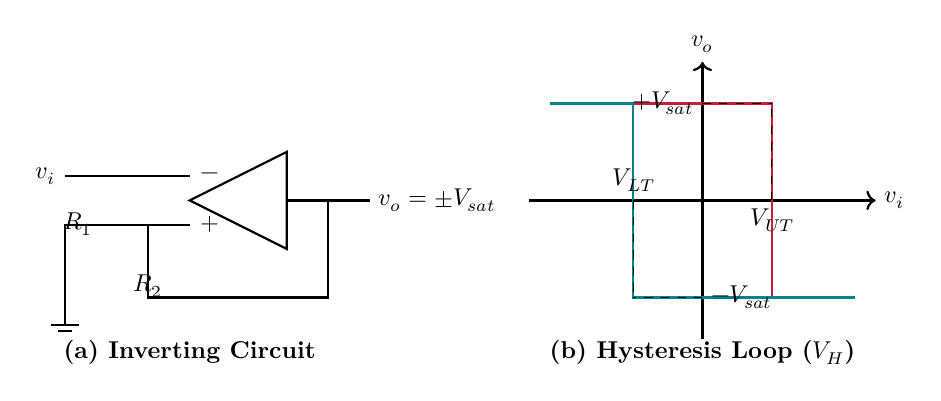
\begin{tikzpicture}[scale=0.88, transform shape]
  % Circuit
  \begin{scope}[shift={(-4.2, 0)}]
    \draw[thick] (0, 0) -- (1.4, 0.7) -- (1.4, -0.7) -- cycle;
    \node at (0.3, 0.35) {$-$}; \node at (0.3, -0.35) {$+$};

    \draw[thick] (0, 0.35) -- (-1.8, 0.35) node[left] {$v_i$};
    \draw[thick] (1.4, 0) -- (2.6, 0) node[right] {$v_o = \pm V_{sat}$};

    % Positive feedback
    \draw[thick] (0, -0.35) -- (-0.6, -0.35) -- (-0.6, -1.4) to[rectangle, draw=myteal, fill=hdrteal, minimum width=0.8cm, minimum height=0.4cm] (0.8, -1.4) node[midway, below=2pt] {$R_2$} -- (2.0, -1.4) -- (2.0, 0);
    \draw[thick] (-0.6, -0.35) -- (-1.8, -0.35) to[rectangle, draw=myteal, fill=hdrteal, minimum width=0.4cm, minimum height=0.8cm] (-1.8, -1.4) node[midway, left=2pt] {$R_1$} -- (-1.8, -1.8);
    \draw[thick] (-2.0, -1.8) -- (-1.6, -1.8);
    \draw[thick] (-1.9, -1.88) -- (-1.7, -1.88);
    \node at (0, -2.2) [font=\bfseries] {(a) Inverting Circuit};
  \end{scope}

  % Hysteresis loop
  \begin{scope}[shift={(3.2, 0)}]
    \draw[thick, ->] (-2.5, 0) -- (2.5, 0) node[right] {$v_i$};
    \draw[thick, ->] (0, -2.0) -- (0, 2.0) node[above] {$v_o$};

    \draw[thick, color=myred] (-2.2, 1.4) -- (1.0, 1.4) -- (1.0, -1.4) -- (2.2, -1.4);
    \draw[thick, color=myteal] (2.2, -1.4) -- (-1.0, -1.4) -- (-1.0, 1.4) -- (-2.2, 1.4);

    \draw[dashed] (1.0, 0) node[below] {$V_{UT}$} -- (1.0, 1.4);
    \draw[dashed] (-1.0, 0) node[above] {$V_{LT}$} -- (-1.0, -1.4);
    \draw[dashed] (0, 1.4) node[left] {$+V_{sat}$} -- (1.0, 1.4);
    \draw[dashed] (0, -1.4) node[right] {$-V_{sat}$} -- (-1.0, -1.4);

    \node at (0, -2.2) [font=\bfseries] {(b) Hysteresis Loop ($V_H$)};
  \end{scope}
\end{tikzpicture}
\end{tcolorbox}

\begin{tcolorbox}[formulabox, title={Threshold and Hysteresis Equations}]
For symmetric supply voltages $\pm V_{sat}$:
\begin{equation}
  V_{UT} = +\frac{R_1}{R_1 + R_2} V_{sat}, \qquad V_{LT} = -\frac{R_1}{R_1 + R_2} V_{sat}
\end{equation}
The Hysteresis Width $V_H$ is given by:
\begin{equation}
  V_H = V_{UT} - V_{LT} = 2\,\frac{R_1}{R_1 + R_2} V_{sat}
\end{equation}
\textbf{Applications}:
\begin{enumerate}[leftmargin=14pt, itemsep=2pt, topsep=2pt]
  \item Clean digital clock recovery from distorted or noisy analog sine waves.
  \item Astable relaxation square-wave oscillators.
  \item Debouncing mechanical tactile switches.
\end{enumerate}
\end{tcolorbox}

% ─── Section 4: Active Filters ────────────────────────────────────────────────
\section{Active Filters}

\begin{tcolorbox}[defbox, title={Definition: Active Filter}]
An \textbf{Active Filter} is a frequency-selective network employing active elements (typically op-amps) combined with passive resistors and capacitors, completely eliminating the need for bulky, lossy inductors at low and medium frequencies ($< 1\text{ MHz}$).
\end{tcolorbox}

\subsection{Filter Approximation Functions}
\begin{itemize}[leftmargin=12pt, itemsep=3pt, topsep=2pt]
  \item \textbf{Butterworth}: Maximally flat passband response; zero passband ripple; smooth roll-off at $-20n\text{ dB/decade}$ where $n$ is the filter order.
  \item \textbf{Chebyshev}: Steeper transition skirt at the expense of predetermined passband ripple ($\epsilon$).
  \item \textbf{Bessel}: Maximally flat group delay (linear phase); preserves waveform shapes without ringing or overshoot.
\end{itemize}

\subsection{First and Second-Order Sallen-Key Low-Pass Filters (LPF)}
\begin{tcolorbox}[defbox, title={Sallen--Key Filter}]
A \textbf{Sallen--Key filter} is an active filter stage that uses an $RC$ network and a non-inverting amplifier or buffer. Its low-pass form passes low frequencies and attenuates frequencies above the cutoff.
\end{tcolorbox}

\begin{tcolorbox}[formulabox, title={1st-Order Active LPF}]
Transfer function:
\begin{equation}
  H(s) = \frac{A_F}{1 + s/\omega_c}, \qquad f_c = \frac{1}{2\pi R C}, \qquad A_F = 1 + \frac{R_f}{R_1}
\end{equation}
Roll-off in stopband is $-20\text{ dB/decade}$ ($-6\text{ dB/octave}$).
\end{tcolorbox}

\begin{tcolorbox}[tikzbox, title={Second-Order Sallen-Key Low-Pass Filter Topology}]
\centering
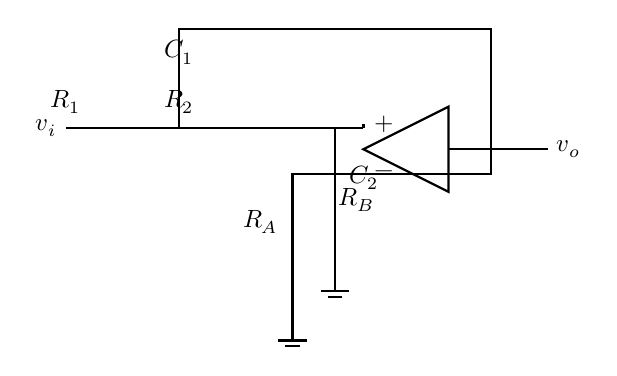
\begin{tikzpicture}[scale=0.9, transform shape]
  \draw[thick] (0, 0) node[left] {$v_i$} to[rectangle, draw=myteal, fill=hdrteal, minimum width=0.8cm, minimum height=0.4cm] (1.2, 0) node[midway, above=2pt] {$R_1$} -- (2.0, 0) to[rectangle, draw=myteal, fill=hdrteal, minimum width=0.8cm, minimum height=0.4cm] (3.2, 0) node[midway, above=2pt] {$R_2$} -- (4.2, 0);

  % Opamp
  \draw[thick] (4.2, -0.3) -- (5.4, 0.3) -- (5.4, -0.9) -- cycle;
  \node at (4.5, 0.05) {$+$}; \node at (4.5, -0.65) {$-$};
  \draw[thick] (4.2, 0) -- (4.2, 0.05);

  % Capacitor C2 to ground
  \draw[thick] (3.8, 0) -- (3.8, -1.4) to[rectangle, draw=myred, fill=hdrred, minimum width=0.7cm, minimum height=0.35cm] (3.8, -1.9) node[midway, right=2pt] {$C_2$} -- (3.8, -2.3);
  \draw[thick] (3.6, -2.3) -- (4.0, -2.3);
  \draw[thick] (3.7, -2.38) -- (3.9, -2.38);

  % Feedback Capacitor C1
  \draw[thick] (1.6, 0) -- (1.6, 1.4) to[rectangle, draw=myred, fill=hdrred, minimum width=0.7cm, minimum height=0.35cm] (3.8, 1.4) node[midway, above=2pt] {$C_1$} -- (6.0, 1.4) -- (6.0, -0.3);

  % Opamp output
  \draw[thick] (5.4, -0.3) -- (6.8, -0.3) node[right] {$v_o$};

  % Feedback resistors RA, RB
  \draw[thick] (4.2, -0.65) -- (3.2, -0.65) -- (3.2, -2.0) to[rectangle, draw=myteal, fill=hdrteal, minimum width=0.4cm, minimum height=0.7cm] (3.2, -2.7) node[midway, left=2pt] {$R_A$} -- (3.2, -3.0);
  \draw[thick] (3.0, -3.0) -- (3.4, -3.0);
  \draw[thick] (3.1, -3.08) -- (3.3, -3.08);
  \draw[thick] (3.2, -0.65) -- (5.0, -0.65) to[rectangle, draw=myteal, fill=hdrteal, minimum width=0.8cm, minimum height=0.4cm] (5.8, -0.65) node[midway, below=2pt] {$R_B$} -- (6.0, -0.65) -- (6.0, -0.3);
\end{tikzpicture}
\end{tcolorbox}

\begin{tcolorbox}[formulabox, title={2nd-Order Sallen-Key LPF Transfer Function and Design Equations}]
By applying Kirchhoff's Current Law at internal nodes:
\begin{equation}
  H(s) = \frac{v_o(s)}{v_i(s)} = \frac{A_F \omega_0^2}{s^2 + s \left(\frac{\omega_0}{Q}\right) + \omega_0^2}
\end{equation}
where:
\begin{equation}
  \omega_0 = \frac{1}{\sqrt{R_1 R_2 C_1 C_2}}, \qquad A_F = 1 + \frac{R_B}{R_A}
\end{equation}
For equal components $R_1 = R_2 = R$ and $C_1 = C_2 = C$:
\begin{equation}
  f_0 = \frac{1}{2\pi R C}, \qquad Q = \frac{1}{3 - A_F}
\end{equation}
\textbf{Butterworth Condition ($Q = 0.7071$)}:
\begin{equation}
  3 - A_F = \sqrt{2} \implies A_F = 3 - \sqrt{2} \approx 1.586 \implies \frac{R_B}{R_A} = 0.586
\end{equation}
Stopband roll-off is $-40\text{ dB/decade}$ ($-12\text{ dB/octave}$).
\end{tcolorbox}

\subsection{Second-Order Sallen-Key High-Pass Filter (HPF)}
Obtained by swapping the positions of resistors and capacitors in the Sallen-Key topology:
\begin{tcolorbox}[formulabox, title={2nd-Order Sallen-Key HPF Transfer Function}]
\begin{equation}
  H(s) = \frac{A_F s^2}{s^2 + s \left(\frac{\omega_0}{Q}\right) + \omega_0^2}
\end{equation}
with $f_0 = \frac{1}{2\pi R C}$ and $A_F = 1.586$ for maximally flat Butterworth response. Stopband attenuation rolls off at $+40\text{ dB/decade}$ below $f_0$.
\end{tcolorbox}

\subsection{Band-Pass and Band-Stop Filters}
\begin{itemize}[leftmargin=12pt, itemsep=3pt, topsep=2pt]
  \item \textbf{Multiple-Feedback (MFB) Band-Pass Filter}: Employs an inverting configuration with two feedback paths (one resistive, one capacitive). Provides stable, high-Q center frequency $f_0 = \frac{1}{2\pi C \sqrt{(R_1 \parallel R_2) R_3}}$.
  \item \textbf{Active Twin-T Notch Filter}: Rejects a single narrow frequency notch ($f_0 = \frac{1}{2\pi R C}$) while passing all other frequencies. Active bootstrapping via an op-amp follower sharpens the notch depth and increases the effective $Q$ factor up to 50.
\end{itemize}

% ─── Section 5: Quick Revision Page ───────────────────────────────────────────
\newpage
\begin{center}
  {\large\bfseries\color{myred} Quick Revision --- Module 4}\\[3pt]
  {\small\color{mydark} Differential Amplifiers and Op-Amp Applications $|$ EC402}
\end{center}
\noindent{\color{myred}\rule{\linewidth}{1.2pt}}
\vspace{4pt}

\begin{tcolorbox}[formulabox, title={Key Formulas at a Glance}]
\small
\renewcommand{\arraystretch}{1.35}
\setlength{\tabcolsep}{5pt}
\noindent\begin{tabularx}{\linewidth}{B{4.1cm}Y}
Diff Amp Gain & $A_d = -g_m R_C = -\frac{I_{EE} R_C}{2 V_T}$ \newline $A_c \approx -\frac{R_C}{2 R_E}$ \\[3pt]
Common Mode Rejection Ratio & $\text{CMRR} = \left|A_d/A_c\right|$ \newline $\text{CMRR} \approx 2g_m R_E = I_{EE}R_E/V_T$ \newline $\text{CMRR}_{\text{dB}} = 20\log_{10}(\text{CMRR})$ \\[3pt]
Input Common-Mode Range & $V_{icm,\max} = V_{CC} - \frac{I_{EE}R_C}{2} + 0.7\text{ V}$ \newline $V_{icm,\min} = -V_{EE} + V_{CS} + 0.7\text{ V}$ \\[3pt]
Op-Amp Gain & Inverting $A_v = -\frac{R_f}{R_1}$ \newline Non-Inverting $A_v = 1 + \frac{R_f}{R_1}$ \\[3pt]
Slew Rate \& Bandwidth & $\text{SR} = \left.\frac{dv_o}{dt}\right|_{\max} = \frac{I_{EE}}{C_c}$ \newline $f_{\max} = \frac{\text{SR}}{2\pi V_m}$ \\[3pt]
Instrumentation Amp & $v_o = \left(1 + \frac{2 R_1}{R_G}\right)\frac{R_3}{R_2}(v_2 - v_1)$ \\[3pt]
Lossy Integrator & $H(s) = -\frac{R_f/R_1}{1 + s R_f C}$ \newline $f_a = \frac{1}{2\pi R_f C}$ \newline integration band $f \ge 10 f_a$ \\[3pt]
Schmitt Trigger Hysteresis & $V_H = V_{UT} - V_{LT} = 2\,\frac{R_1}{R_1 + R_2} V_{sat}$ \\[3pt]
2nd-Order Sallen-Key LPF & $f_0 = \frac{1}{2\pi RC}$ \newline Butterworth gain $A_F = 1.586$ ($Q = 0.707$)
\end{tabularx}\par
\end{tcolorbox}

\begin{tcolorbox}[defbox, title={One-Line Definitions}, title after break={One-Line Definitions (contd.)}]
\small
\interlinepenalty=10000
\begin{itemize}[leftmargin=1.5em, topsep=2pt, itemsep=4pt]
  \item \textbf{CMRR}: The common-mode rejection ratio is $\lvert A_d/A_c\rvert$, where $A_d$ is differential gain and $A_c$ is common-mode gain. A higher ratio means better rejection of signals common to both inputs.
  \item \textbf{Virtual Ground}: A node held at nearly ground voltage by negative feedback, without a direct connection to ground. In an inverting op-amp circuit, this occurs when the non-inverting input is grounded and the amplifier is operating linearly.
  \item \textbf{Slew Rate}: The maximum rate at which the op-amp output voltage can change, usually given in volts per microsecond.
  \item \textbf{Input Offset Voltage}: The differential DC voltage that must be applied between op-amp inputs to force output to zero.
  \item \textbf{Lossy Integrator}: An op-amp integrator with a resistor in parallel with its feedback capacitor to keep the DC gain finite.
  \item \textbf{Schmitt Trigger}: A comparator that uses positive feedback to set different switching thresholds for rising and falling input voltages.
  \item \textbf{Hysteresis}: In a Schmitt trigger, the output inside the threshold band depends on its previous state. The hysteresis width is the difference between the upper and lower thresholds.
  \item \textbf{Butterworth Filter}: A filter designed for a maximally flat passband magnitude response.
\end{itemize}
\end{tcolorbox}

\begin{tcolorbox}[exambox, title={Frequently Asked / Viva Questions}]
\begin{enumerate}[topsep=0pt, label=\textbf{Q\arabic*.}, itemsep=5pt]
  \item \Q{Why is an active current mirror preferred over a resistor in the emitter tail of a diff amp?}
  An active current mirror provides very high dynamic resistance ($r_o$ in M$\Omega$ range) while requiring negligible DC voltage drop, boosting CMRR to $> 100\text{ dB}$ without restricting supply rails.

  \item \Q{What causes the phenomenon of virtual ground in an op-amp circuit?}
  Since open-loop gain $A_{OL} \to \infty$ and output voltage $v_o$ is finite, the differential input voltage $v_d = v_+ - v_- = v_o / A_{OL} \to 0$. When $v_+$ is connected to ground ($0\text{ V}$), $v_-$ is forced to $0\text{ V}$.

  \item \Q{What is the primary drawback of an ideal op-amp integrator?}
  At DC ($\omega = 0$), capacitor impedance is infinite, causing the op-amp to run in open loop ($A_v \approx 10^5$). Tiny DC offset voltages saturate the output to the supply rail.

  \item \Q{How does a lossy integrator overcome output saturation?}
  By shunting a feedback resistor $R_f$ across capacitor $C$. At DC, the capacitor is open-circuit, setting a finite DC closed-loop gain $A_v(0) = -R_f/R_1$.

  \item \Q{What is the function of the level shifter stage inside an IC op-amp?}
  Because op-amp internal stages are direct-coupled, DC quiescent levels drift upwards toward $+V_{CC}$. The level shifter shifts the quiescent DC output level precisely to $0\text{ V}$.

  \item \Q{Why does a differentiator have stability issues at high frequencies?}
  Gain increases at $+20\text{ dB/decade}$ with frequency, amplifying high-frequency noise and introducing a $90^\circ$ phase lead that erodes phase margin, leading to spurious oscillation.

  \item \Q{Explain the role of hysteresis in a Schmitt trigger.}
  Hysteresis prevents high-frequency input noise from causing unwanted false transitions when the signal crosses the switching threshold.

  \item \Q{What is the 3-op-amp instrumentation amplifier's key advantage over a single op-amp diff amp?}
  Both inputs connect directly to non-inverting op-amp terminals, guaranteeing extremely high input impedance ($> 10^9\,\Omega$), while gain is tuned via a single floating resistor $R_G$.

  \item \Q{What condition must be satisfied for a 2nd-order Sallen-Key filter to achieve Butterworth response?}
  The quality factor must be $Q = 1/\sqrt{2} \approx 0.7071$, which dictates that passband gain $A_F = 3 - \sqrt{2} = 1.586$ ($R_B/R_A = 0.586$).

  \item \Q{What is Full-Power Bandwidth ($f_{\max}$)?}
  The maximum operating frequency at which an op-amp can deliver its rated maximum peak output voltage without experiencing slew-rate distortion: $f_{\max} = \frac{\text{SR}}{2\pi V_m}$.
\end{enumerate}
\end{tcolorbox}

\begin{tcolorbox}[tikzbox, title={Summary Comparison of Active Filter Topologies}]
\renewcommand{\arraystretch}{1.25}
\setlength{\tabcolsep}{5pt}
\noindent\begin{tabularx}{\linewidth}{|B{3.2cm}|B{2.8cm}|B{2.8cm}|Y|}
\hline
\textbf{Filter Topology} & \textbf{Cutoff / Center Freq} & \textbf{Passband Gain} & \textbf{Key Features \& Trade-offs} \\
\hline
1st-Order Sallen-Key LPF & $f_c = \frac{1}{2\pi RC}$ & $A_F = 1 + \frac{R_f}{R_1}$ & $-20\text{ dB/dec}$ roll-off; simple, unconditionally stable. \\
\hline
2nd-Order Sallen-Key LPF & $f_0 = \frac{1}{2\pi RC}$ & $A_F = 1.586$ (Butterworth) & $-40\text{ dB/dec}$ roll-off; sharp knee; low component count. \\
\hline
2nd-Order Sallen-Key HPF & $f_0 = \frac{1}{2\pi RC}$ & $A_F = 1.586$ & $+40\text{ dB/dec}$ attenuation in stopband; high-pass filtering. \\
\hline
MFB Band-Pass Filter & $f_0 = \frac{1}{2\pi C \sqrt{R_{eq} R_3}}$ & $A_0 = -\frac{R_3}{2 R_1}$ & Inverting, stable high-$Q$ operation; low sensitivity to op-amp GBW. \\
\hline
Active Twin-T Notch & $f_0 = \frac{1}{2\pi RC}$ & Unity ($0\text{ dB}$) & High-$Q$ deep notch rejection; active bootstrap sharpens null depth. \\
\hline
\end{tabularx}\par
\end{tcolorbox}


\end{document}
